\usepackage{ifthen}
\usepackage{graphicx}
\usepackage{booktabs}
\usepackage{tabularx}
\usepackage{algorithm}
%\usepackage{algorithmx}
%\usepackage{cwpuzzle}
\usepackage{algpseudocode}
\usepackage[english]{babel}
%\usepackage{qtree}
\usepackage{amssymb}
\usepackage{amsmath,amsthm}
\usepackage{subcaption}
\usepackage{mathrsfs}
%\usepackage{eurosym}
\usepackage{soul}
\usepackage{fontawesome}
\usepackage{etoolbox}
\usepackage{soul}
\usepackage{multicol}
\usepackage{listings}
\usepackage{color}

\definecolor{mygreen}{rgb}{0,0.6,0}
\definecolor{mygray}{rgb}{0.5,0.5,0.5}
\definecolor{mymauve}{rgb}{0.58,0,0.82}
\usepackage{tikz}
\usepackage{xstring}
\usepackage{pgfplots}
\usepackage{etoolbox}
\usepackage{ifthen}
\usetikzlibrary{arrows,shapes}
\usetikzlibrary{positioning, calc}

\definecolor{hospital}{RGB}{0,0,255}
\definecolor{patient}{RGB}{255,0,0}

\tikzstyle{flow_node}=[circle,draw=black,minimum size=15pt,inner sep=0pt]
\tikzstyle{flow_s}=[fill=green!20]
\tikzstyle{flow_subtask}=[fill=green!80]
\tikzstyle{flow_task}=[fill=red!80]
\tikzstyle{flow_t}=[fill=blue!20]
\tikzstyle{flow_edge}=[->, ultra thick]
\tikzstyle{flow_capacity}=[fill=white, inner sep = 1pt]
\tikzstyle{flow_edge_mincut}=[draw=red]
\tikzstyle{flow_edge_fullcap}=[draw=red]
\tikzstyle{flow_mincut}=[dashed, thick]
\tikzstyle{flow_supply}=[fill=green!80]
\tikzstyle{flow_demand}=[fill=red!80]

\newcommand\ifMaxFlow[4]{
	\begingroup
		\pgfmathsetmacro{\flow}{#1}
		\pgfmathsetmacro{\cap}{#2}
		\pgfmathparse{ifthenelse(\flow == \cap,1,0)}
		\ifdim\pgfmathresult pt= 1 pt
			 #3
			\else
			 #4
		\fi
	\endgroup
}

\newcommand\ifSomeFlow[3]{
	\begingroup
		\pgfmathsetmacro{\flow}{#1}
		\pgfmathparse{ifthenelse(\flow > 0,1,0)}
		\ifdim\pgfmathresult pt= 1 pt
			 #2
			\else
			 #3
		\fi
	\endgroup
}


\usepackage[duration=105,lastminutes=15]{../common/pdfpcnotes}

\makeatletter
\let\@@magyar@captionfix\relax
\makeatother

\newcommand{\bigO}{O}

\usetheme[width=0mm]{PaloAlto}
\setbeamertemplate{navigation symbols}
{\ifthenelse{\not\equal{\thepage}{1}}
  {\insertframenumber}
  {}
}
\setbeamertemplate{footline}%
{\ifthenelse{\not\equal{\thepage}{1}}%
  {\color{gray!30!white}{\tiny \copyright 2018 TU Delft}}% \hfill\insertframenumber/\inserttotalframenumber}
  {}
}

\newenvironment<>{problemblock}[1]{%
  \begin{actionenv}#2%
      \def\insertblocktitle{Problem: #1}%
      \par%
      \mode<presentation>{%
        \setbeamercolor{block title}{fg=white,bg=orange!80!black}
       \setbeamercolor{block body}{fg=black,bg=orange!40}
       \setbeamercolor{itemize item}{fg=orange!20!black}
       \setbeamertemplate{itemize item}[triangle]
     }%
      \usebeamertemplate{block begin}}
    {\par\usebeamertemplate{block end}\end{actionenv}}

\newenvironment<>{questionblock}[1]{%
  \begin{actionenv}#2%
      \def\insertblocktitle{Question: #1}%
      \par%
      \mode<presentation>{%
        \setbeamercolor{block title}{fg=white,bg=cyan!80!black}
       \setbeamercolor{block body}{fg=black,bg=cyan!30}
       \setbeamercolor{itemize item}{fg=cyan!20!black}
       \setbeamertemplate{itemize item}[triangle]
     }%
      \usebeamertemplate{block begin}}
    {\par\usebeamertemplate{block end}\end{actionenv}}

\newenvironment<>{answerblock}[1]{%
  \begin{actionenv}#2%
      \def\insertblocktitle{Answer: #1}%
      \par%
      \mode<presentation>{%
        \setbeamercolor{block title}{fg=white,bg=green!80!black}
       \setbeamercolor{block body}{fg=black,bg=green!30}
       \setbeamercolor{itemize item}{fg=green!20!black}
       \setbeamertemplate{itemize item}[triangle]
     }%
      \usebeamertemplate{block begin}}
    {\par\usebeamertemplate{block end}\end{actionenv}}

% Fix a bug in lstlinebgrd
% https://tex.stackexchange.com/questions/451532/recent-issues-with-lstlinebgrd-package-with-listings-after-the-latters-updates

\makeatletter
\let\old@lstKV@SwitchCases\lstKV@SwitchCases
\def\lstKV@SwitchCases#1#2#3{}
\makeatother
\usepackage{lstlinebgrd}
\makeatletter
\let\lstKV@SwitchCases\old@lstKV@SwitchCases

\lst@Key{numbers}{none}{%
    \def\lst@PlaceNumber{\lst@linebgrd}%
    \lstKV@SwitchCases{#1}%
    {none:\\%
     left:\def\lst@PlaceNumber{\llap{\normalfont
                \lst@numberstyle{\thelstnumber}\kern\lst@numbersep}\lst@linebgrd}\\%
     right:\def\lst@PlaceNumber{\rlap{\normalfont
                \kern\linewidth \kern\lst@numbersep
                \lst@numberstyle{\thelstnumber}}\lst@linebgrd}%
    }{\PackageError{Listings}{Numbers #1 unknown}\@ehc}}
\makeatother

\lstset{ 
  backgroundcolor=\color{white},   % choose the background color; you must add \usepackage{color} or \usepackage{xcolor}; should come as last argument
  basicstyle=\footnotesize\ttfamily,        % the size of the fonts that are used for the code
  breakatwhitespace=false,         % sets if automatic breaks should only happen at whitespace
  breaklines=true,                 % sets automatic line breaking
  captionpos=b,                    % sets the caption-position to bottom
  commentstyle=\color{mygreen},    % comment style
  deletekeywords={...},            % if you want to delete keywords from the given language
	escapeinside={\%*}{*\%},          % if you want to add LaTeX within your code
  extendedchars=true,              % lets you use non-ASCII characters; for 8-bits encodings only, does not work with UTF-8
  frame=single,	                   % adds a frame around the code
  keepspaces=true,                 % keeps spaces in text, useful for keeping indentation of code (possibly needs columns=flexible)
  keywordstyle=\color{blue},       % keyword style
  language=Python,                 % the language of the code
	literate={\ \ }{{\ }}1,					 % Replace two spaces with just one
  morekeywords={*,...},            % if you want to add more keywords to the set
  numbers=left,                    % where to put the line-numbers; possible values are (none, left, right)
  numbersep=5pt,                   % how far the line-numbers are from the code
  numberstyle=\tiny\color{mygray}, % the style that is used for the line-numbers
  rulecolor=\color{black},         % if not set, the frame-color may be changed on line-breaks within not-black text (e.g. comments (green here))
  showspaces=false,                % show spaces everywhere adding particular underscores; it overrides 'showstringspaces'
  showstringspaces=false,          % underline spaces within strings only
  showtabs=false,                  % show tabs within strings adding particular underscores
  stepnumber=1,                    % the step between two line-numbers. If it's 1, each line will be numbered
  stringstyle=\color{mymauve},     % string literal style
  tabsize=2,   	                   % sets default tabsize to 2 spaces
	emptylines=*1
}
\lstset{
	defaultdialect=[LaTeX]TeX
}

%%%%%%%%%%%%%%%%%%%%%%%%%%%%%%%%%%%%%%%%%%%%%%%%%%%%%%%%%%%%%%%%%%%%%%%%%%%%%%%%
% Hacks for highlighting lines in listings, thanks to Robbert Krebbers
%%%%%%%%%%%%%%%%%%%%%%%%%%%%%%%%%%%%%%%%%%%%%%%%%%%%%%%%%%%%%%%%%%%%%%%%%%%%%%%%

\makeatletter
\newlength\beamerleftmargin
\setlength\beamerleftmargin{\Gm@lmargin}
\makeatother

\makeatletter
\newcount\bt@rangea
\newcount\bt@rangeb

\newcommand\btIfInRange[2]{%
    \global\let\bt@inrange\@secondoftwo%
    \edef\bt@rangelist{#2}%
    \foreach \range in \bt@rangelist {%
        \afterassignment\bt@getrangeb%
        \bt@rangea=0\range\relax%
        \pgfmathtruncatemacro\result{ ( #1 >= \bt@rangea) && (#1 <= \bt@rangeb) }%
        \ifnum\result=1\relax%
            \breakforeach%
            \global\let\bt@inrange\@firstoftwo%
        \fi%
    }%
    \bt@inrange%
}
\newcommand\bt@getrangeb{%
    \@ifnextchar\relax%
        {\bt@rangeb=\bt@rangea}%
        {\@getrangeb}%
}
\def\@getrangeb-#1\relax{%
    \ifx\relax#1\relax%
        \bt@rangeb=100000%   \maxdimen is too large for pgfmath
    \else%
        \bt@rangeb=#1\relax%
    \fi%
}

\newcommand<>{\btLstHL}[1]{%
  \only#2{\btIfInRange{\value{lstnumber}}{#1}%
    {\color{blue!30}}%
    {\def\lst@linebgrdcmd####1####2####3{}}% define as no-op
  }%
}%
\makeatother



\title[Algorithms \& Data Structures]{TI1520TW Algorithms \& Data Structures}
\subtitle{\color{cyan} \textbf{Lecture 5: Stacks \& Queues}}
\author{Stefan Hugtenburg\\ {\tiny{\qquad~~\copyright 2019 TU Delft}}}
\institute{CSE Teaching Team | EEMCS | TU Delft}
\titlegraphic{
\includegraphics[height=1cm]{../common/logo.pdf}~\hfill~
\includegraphics[height=1cm]{../common/cc-by-nc-sa.png}}
\date{2018-2019 Q3}

\begin{document}

\frame{\titlepage}

\section{Introduction}

\begin{frame}
	\frametitle{You are here.}
	\begin{block}{The course so far}
		\begin{itemize}
			\item Time and Space complexity
			\item Lists, Stacks, and Queues
			\item Sorting
		\end{itemize}
	\end{block}
	\pause
	\begin{exampleblock}{Today's content}
		\begin{itemize}
			\item Trees!
			\item Properties and traversals
		\end{itemize}
	\end{exampleblock}
	\pause
	\begin{block}{The future}
		\begin{itemize}
			\item Heaps and Search Trees
			\item Maps, Sets, and Graphs
			\item P vs NP\dots
		\end{itemize}
	\end{block}
\end{frame}


\begin{frame}
	\frametitle{Some small updates}
	\begin{itemize}
		\item Grading of week 1. Sorry we were so late!
		\item We hope to be a lot earlier this week!
			\pause
		\item I will try to generate hand-out versions of my slides as well (less clicking/scrolling).
		\item My slides always end with what sections of the book they correspond to :)
			\pause
		\item FBF fixed the broken links, but now other stuff seems to be broken..
			\pause
		\item You have only a few more days to register for the exams!
		\item Two practice exams will be available by the end of the week (one analysis, one implementation).
			\pause
		\item Again, remember that you can render TeX in WebLab.
	\end{itemize}
\end{frame}

\section{Lists Recap}
\label{sec:lists_recap}

\begin{frame}
	\frametitle{Doubly-Linked Lists}
		\begin{columns}
			\column{0.655\textwidth}
		\begin{center}
			\begin{tikzpicture}[scale=0.85, transform shape]
	\foreach \x/\val in {0/1,1/20,2/42,3/189,4/\alt<5>{\alert{4242}}{17},5/-2}{
	\node[draw,rectangle, fill=gray!10, minimum size =1cm] (c) at (\x,0) {\val};
	\node[olive] (index) at (\x,-1) {\x};
}
\node[] at (-2,0) {Array:};
\node[] at (-2,-1) {Indices:};
\end{tikzpicture}

		\end{center}
			\column{0.355\textwidth}
			\begin{block}{An array}
				A block of memory, index-based.
			\end{block}	
		\end{columns}
		\pause
		\begin{columns}
			\column{0.655\textwidth}
		\begin{center}
			% Tikz template taken from: https://tex.stackexchange.com/a/19288
\begin{tikzpicture}[list/.style={rectangle split, rectangle split parts=2,
    draw, rectangle split horizontal}, >=stealth, start chain]

  \node[list,on chain] (A) {42};
  \node[list,on chain] (B) {99};
  \draw[*->] let \p1 = (A.two), \p2 = (A.center) in (\x1,\y2) -- (B);
  \node[list,on chain] (C) {12};
  \draw[*->] let \p1 = (B.two), \p2 = (B.center) in (\x1,\y2) -- (C);
  \node[on chain,draw,inner sep=6pt] (D) {};
  \draw (D.north east) -- (D.south west);
  \draw (D.north west) -- (D.south east);
  \draw[*->] let \p1 = (C.two), \p2 = (C.center) in (\x1,\y2) -- (D);

\end{tikzpicture}	

		\end{center}
			\column{0.355\textwidth}
			\begin{block}{A singly linked list}
				Only has connections in one direction.	
			\end{block}	
		\end{columns}
		\pause
		\begin{columns}
			\column{0.655\textwidth}
				
			\begin{center}
				% Tikz template taken from: https://tex.stackexchange.com/a/19288
\begin{tikzpicture}[list/.style={rectangle split, rectangle split parts=2,
    draw, rectangle split horizontal},start chain]

		\only<2->{
  \node[on chain,draw,inner sep=6pt] (E) {};
  \draw (E.north east) -- (E.south west);
  \draw (E.north west) -- (E.south east);
}
  \node[list,on chain] (A) {42};
  \node[list,on chain] (B) {99};
  \draw[*->] let \p1 = (A.two), \p2 = (A.center) in (\x1,\y2) -- (B);
  \node[list,on chain] (C) {12};
  \draw[*->] let \p1 = (B.two), \p2 = (B.center) in (\x1,\y2) -- (C);
  \node[on chain,draw,inner sep=6pt] (D) {};
  \draw (D.north east) -- (D.south west);
  \draw (D.north west) -- (D.south east);
  \draw[*->] let \p1 = (C.two), \p2 = (C.center) in (\x1,\y2) -- (D);

	\only<2->{
		\draw[->,red,thick] let \p1 = (A.two), \p2 = (A.center) in (B) to [out=150, in=30] (\x1,\y2);
		\draw[->,red,thick] let \p1 = (B.two), \p2 = (B.center) in (C) to [out=150, in=30] (\x1,\y2);
		\draw[->,red,thick] let \p1 = (E.center), \p2 = (E.center) in (A) to [out=150, in=30] (\x1,\y2);
	}
\end{tikzpicture}	

			\end{center}
			\column{0.355\textwidth}
			\begin{block}{A doubly linked list}
				Has connections in both directions.
			\end{block}
				
		\end{columns}
\end{frame}

\begin{frame}
	\frametitle{Remember lists?}
	
	\begin{tabular}{l | c | c | c}
	Operation & Array-based list & SLL & DLL \\	
	\midrule
	Get element $k$ & $O(1)$ &$O(k)$ & $O(k)$ \\
	Insert first element& $O(n)$ & $O(1)$ & $O(1)$\\
	Insert at index $k$& $O(n-k)$ & $O(k)$ & $O(\min(k,n-k))$\\
	Append (amortised)& $O(1)$ & $O(1)$ & $O(1)$\\
	Remove first element& $O(n)$ & $O(1)$ & $O(1)$\\
	Remove last element& $O(1)$ & $O(n)$ & $O(1)$\\
	Remove index $k$& $O(n-k)$ & $O(k)$ & $O(\min(k,n-k))$\\
	Search & $O(n)$ & $O(n)$ & $O(n)$\\
	\end{tabular}

\end{frame}

\section{Stacks}
\label{sec:stacks}

\begin{frame}
	\frametitle{Stacks}
	\begin{center}
		
\includegraphics[width=0.4\textwidth]{figures/stack_of_books.png}\\
		\hspace*{15pt}\hbox{\scriptsize Image from \thinspace{\itshape Pixabay}}
		% https://pixabay.com/en/books-stacked-pile-stacks-25159/
	\end{center}
\end{frame}

\begin{frame}
	\frametitle{Me and my books}
	\framesubtitle{A life-long story}

	\begin{columns}
		\column{0.455\textwidth}
			\begin{center}
				\alt<4->{
					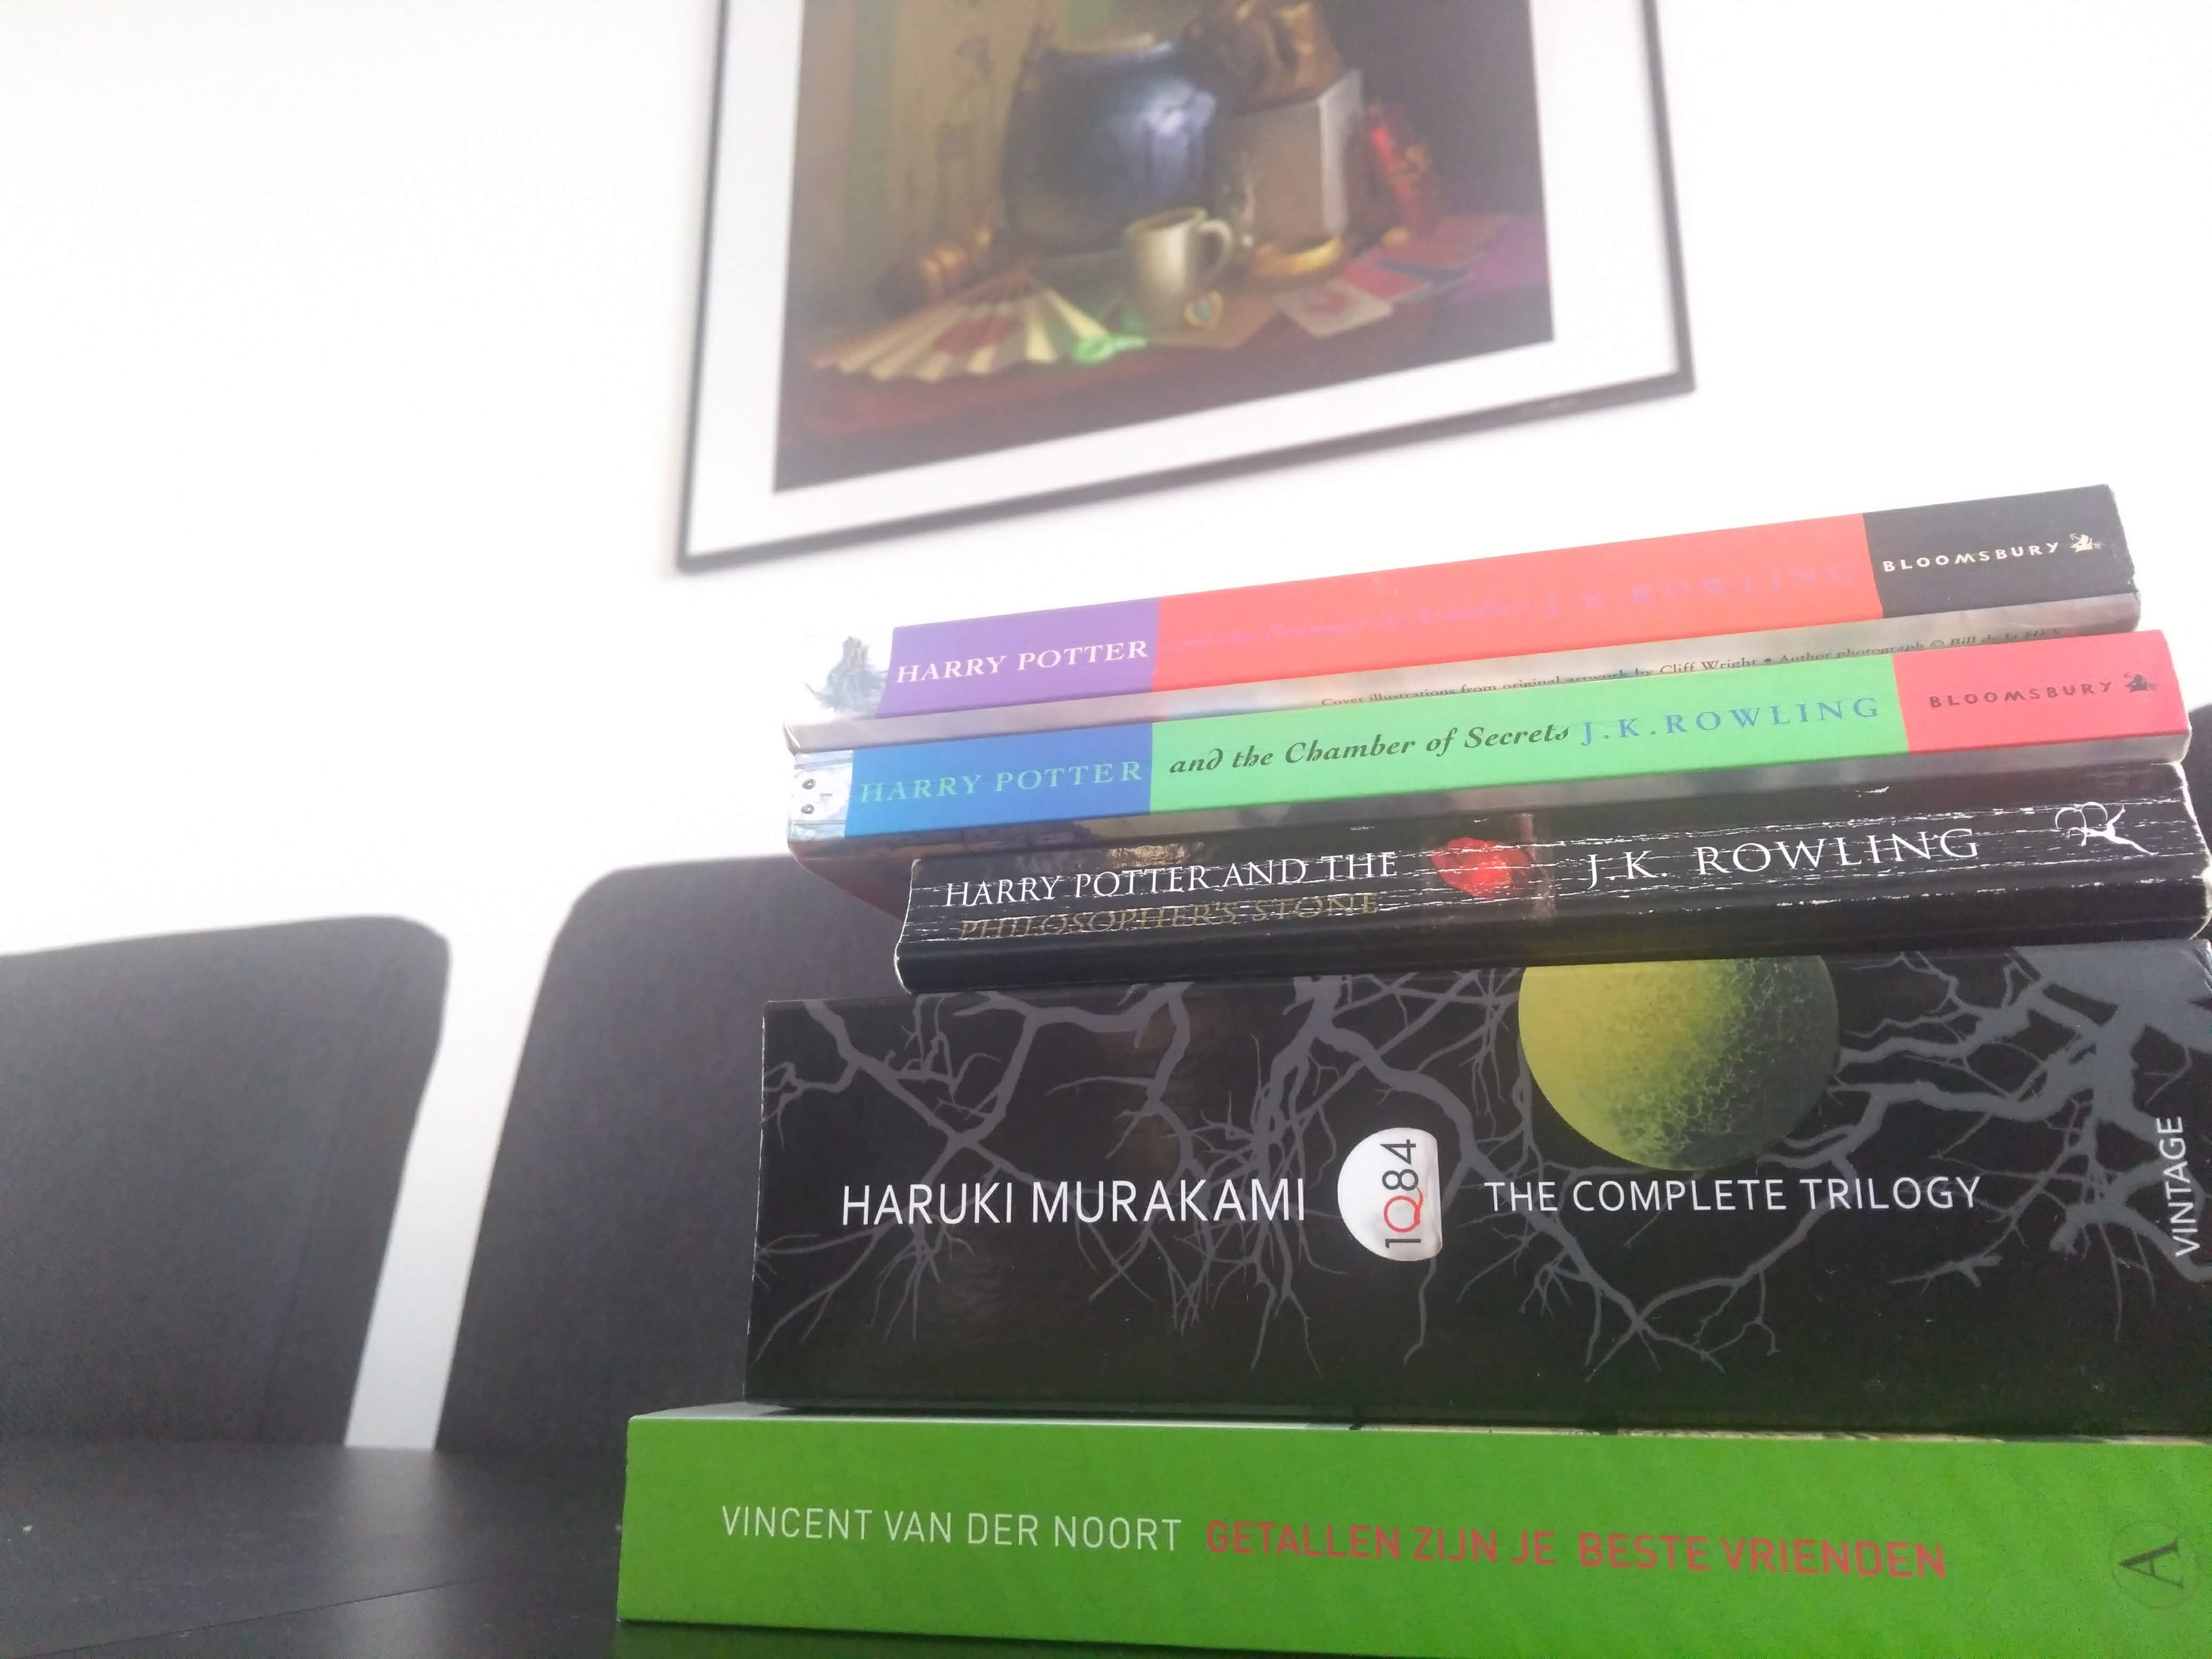
\includegraphics[width=\textwidth]{figures/stack_read.jpg}\\
					}{
					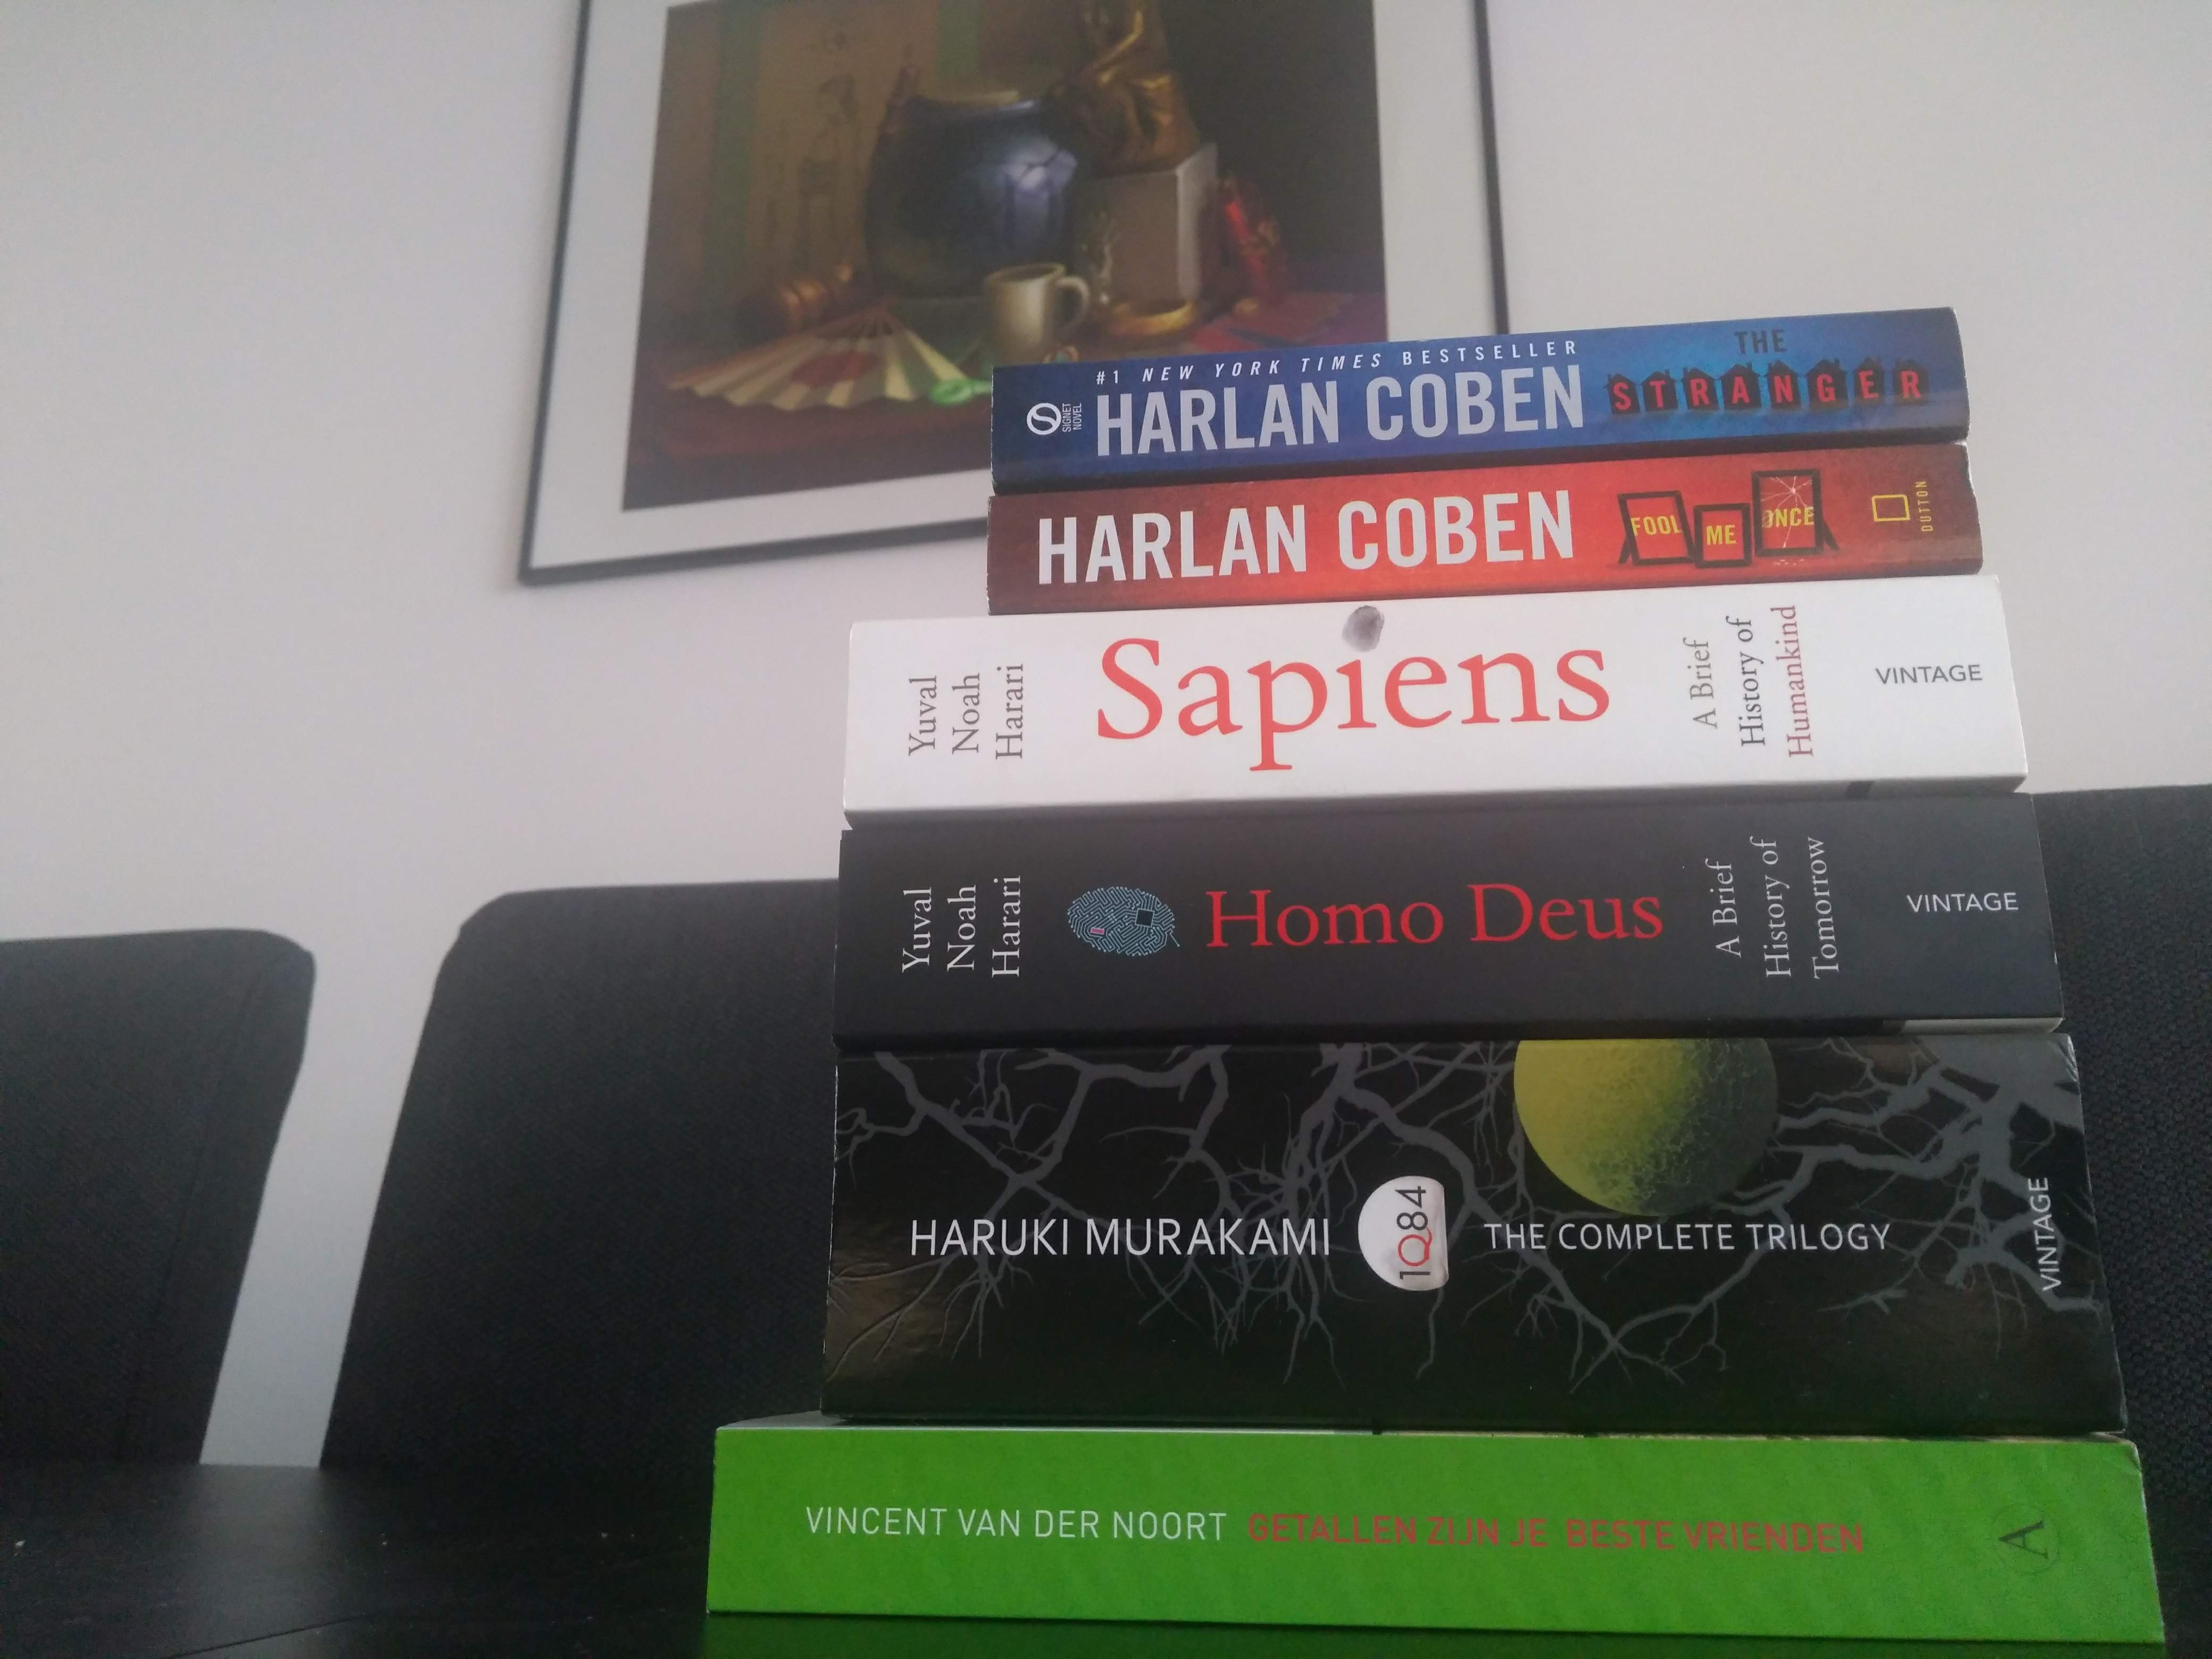
\includegraphics[width=\textwidth]{figures/stack_unread.jpg}\\
					}
				\hspace*{15pt}\hbox{\scriptsize Image By:\thinspace{\itshape Stefan Hugtenburg}}
				\hspace*{15pt}\hbox{\scriptsize Bookcovers and picture in the back by others}
			\end{center}
		\column{0.455\textwidth}
		\begin{itemize}
			\item This is how I used to store books I still wanted to read.
				\pause
			\item A nice \alert{stack} of books, with new ones going on the top.
				\pause
			\item After finishing one, I would take the next one from the top.
				\pause
			\item So after a few weeks\dots
				\pause
			\item This uses the \alert{LIFO}-principle.
		\end{itemize}
	\end{columns}
\end{frame}

\begin{frame}
	\frametitle{The what!?}
	\framesubtitle{LIFO}
	
		\begin{block}{LIFO}
			The \textit{Last-In-First-Out}, or LIFO, principle is the working of a stack.\\
			\pause
			The last thing we've added to the stack is the first thing we take out.\\
			\pause
			Similarly the first we have added to the stack, is the last to be taken out.
		\end{block}	
\end{frame}

\begin{frame}
	\frametitle{The Stack ADT}
	\begin{overlayarea}{\textwidth}{\textheight}
		\only<1>{
			\begin{block}{ADT}
				An ADT, or Abstract Data Type, is a description of the behaviour of a data structure.
			\end{block}	
		}
		\pause
			\begin{block}{The Stack}
				\begin{itemize}
					\item \texttt{size()} (or \texttt{len(s)}) to get the number of items in the stack.
					\item \texttt{push(item)} to add something to the stack.
						\pause
					\item \texttt{pop()} to remove the top element from the stack.
					\item \texttt{top()} to view the top element of the stack.
				\end{itemize}
			\end{block}	
			\pause
			\begin{questionblock}{Data structure?}
				What kind of data structure should we use to implement a Stack?
				\only<4>{
				\begin{enumerate}[A.]
					\item An array
					\item A python list
					\item A linked list
					\item A dict
				\end{enumerate}
			}
			\end{questionblock}
			\pause
			\begin{answerblock}{One end only}
				Only removing and adding on one end? Seems like a DLL will do.
			\end{answerblock}
	\end{overlayarea}
\end{frame}

\begin{frame}
	\frametitle{Implementing a Linked-List based Stack}
	\begin{overlayarea}{\textwidth}{\textheight}
			\begin{tabular}{r | c c}
				Stack operation & DLL operation & Time Complexity \\
				\midrule
				\texttt{size} & \only<2->{\texttt{size} & $O(1)$} \\
				\texttt{push} & \only<2->{\texttt{add\_last} & $O(1)$} \\
				\texttt{pop}  & \only<2->{\texttt{remove\_last} & $O(1)$} \\
				\texttt{top}  & \only<2->{\texttt{tail} & $O(1)$} \\
			\end{tabular}
		
			\begin{columns}[t]
				\column{0.455\textwidth}
			\only<3->{
			\begin{questionblock}{Arrays}
				Could we also do this using an array-based list?	
			\end{questionblock}
		}
			\only<5->{
			\begin{questionblock}{SLL}
				What about an SLL?
			\end{questionblock}
		}
				\column{0.455\textwidth}
				\only<4->{
				\begin{answerblock}{Amortised}
					Sure, but it's only amortised $O(1)$. So why would we?
				\end{answerblock}
				}
				\only<6->{
				\begin{answerblock}{Front = Back}
					Sure, but we add and remove from the front!
				\end{answerblock}
				}
		
			\end{columns}
	\end{overlayarea}
\end{frame}


\section{Use case: Stacks}
\label{sec:use_case_stacks}


\begin{frame}
	\frametitle{Use case: Parsing \LaTeX}
	\begin{columns}
		\column{0.655\textwidth}
		\lstinputlisting[language=TeX]{parseslide.tex}
		\pause
		\column{0.355\textwidth}
		\begin{questionblock}{Testing syntax}
			How can I test this slide will compile?
		\end{questionblock}
		\pause
		\begin{answerblock}{Stacks!}
			By using a Stack!
		\end{answerblock}
	\end{columns}
\end{frame}


\begin{frame}
	\frametitle{An example}
	\begin{columns}
		\column{0.655\textwidth}
		\lstinputlisting[language=TeX,
		 linebackgroundcolor={%
    \btLstHL<1>{1}% on slide 1, highlight lines 1-3
    \btLstHL<2>{3}% on slide 2, highlight lines 6 and 9
    \btLstHL<3>{8}%
    \btLstHL<4>{10}%
    \btLstHL<5>{12}%
    \btLstHL<6>{14}%
    \btLstHL<7>{15}%
    \btLstHL<8>{16}%
  }
		]{parseslide.tex}
		\column{0.355\textwidth}
		\section{Use case: Stacks}
\label{sec:use_case_stacks}


\begin{frame}
	\frametitle{Use case: Parsing \LaTeX}
	\begin{columns}
		\column{0.655\textwidth}
		\lstinputlisting[language=TeX]{parseslide.tex}
		\pause
		\column{0.355\textwidth}
		\begin{questionblock}{Testing syntax}
			How can I test this slide will compile?
		\end{questionblock}
		\pause
		\begin{answerblock}{Stacks!}
			By using a Stack!
		\end{answerblock}
	\end{columns}
\end{frame}


\begin{frame}
	\frametitle{An example}
	\begin{columns}
		\column{0.655\textwidth}
		\lstinputlisting[language=TeX,
		 linebackgroundcolor={%
    \btLstHL<1>{1}% on slide 1, highlight lines 1-3
    \btLstHL<2>{3}% on slide 2, highlight lines 6 and 9
    \btLstHL<3>{8}%
    \btLstHL<4>{10}%
    \btLstHL<5>{12}%
    \btLstHL<6>{14}%
    \btLstHL<7>{15}%
    \btLstHL<8>{16}%
  }
		]{parseslide.tex}
		\column{0.355\textwidth}
		\section{Use case: Stacks}
\label{sec:use_case_stacks}


\input{parseslide.tex}

\begin{frame}
	\frametitle{An example}
	\begin{columns}
		\column{0.655\textwidth}
		\lstinputlisting[language=TeX,
		 linebackgroundcolor={%
    \btLstHL<1>{1}% on slide 1, highlight lines 1-3
    \btLstHL<2>{3}% on slide 2, highlight lines 6 and 9
    \btLstHL<3>{8}%
    \btLstHL<4>{10}%
    \btLstHL<5>{12}%
    \btLstHL<6>{14}%
    \btLstHL<7>{15}%
    \btLstHL<8>{16}%
  }
		]{parseslide.tex}
		\column{0.355\textwidth}
		\input{figures/tikz/parsingtex.tex}\\
		\only<-8>{
		The stack of open \textit{tags}.\\
	}
		\only<9->{
			The code is done and my stack is empty $\to$ Correct TeX.
		}
	\end{columns}
	
\end{frame}

\begin{frame}
	\frametitle{Incorrect Tex}
	\begin{columns}
		\column{0.655\textwidth}
		\lstinputlisting[language=TeX,
		 linebackgroundcolor={%
    \btLstHL<1>{1}% on slide 1, highlight lines 1-3
    \btLstHL<2>{3}% on slide 2, highlight lines 6 and 9
    \btLstHL<3>{5}%
  }
		]{parseerror.tex}
		\column{0.355\textwidth}
		\input{figures/tikz/parsingerror.tex}\\
		The stack of open \textit{tags}.\\
		\only<3->{
			We encounter the wrong closing tag $\to$ Incorrect TeX.
		}
	\end{columns}
\end{frame}

\begin{frame}
	\frametitle{Our TeX parsing algorithm}
	\begin{columns}
		\column{0.655\textwidth}
	\begin{algorithmic}
		\State tagStack $\gets$ empty stack.
		\While{there is TeX}
		\pause
			\If{opening tag}
				\State tagStack.push(tagname)
			\Else
		\pause
			\If{closing tag != tagStack.top()}
				\State \Return False
			\Else
				\State tagStack.pop()
			\EndIf
			\EndIf
		\EndWhile
		\pause
		\State \Return tagStack.size() == 0
	\end{algorithmic}
	\pause
		\column{0.405\textwidth}
			\begin{exampleblock}{Tag based languages}
				This basic syntax checkers, works for any tag-based language!
				\pause
				\begin{itemize}
					\item (La)TeX
					\item HTML
					\item XML
					\item But even for some basics of languages like Java.
				\end{itemize}
				\pause See also \url{https://youtu.be/QZOLb0xHB_Q} to see someone else explain the same thing :)
			\end{exampleblock}	
			
	\end{columns}
\end{frame}
\\
		\only<-8>{
		The stack of open \textit{tags}.\\
	}
		\only<9->{
			The code is done and my stack is empty $\to$ Correct TeX.
		}
	\end{columns}
	
\end{frame}

\begin{frame}
	\frametitle{Incorrect Tex}
	\begin{columns}
		\column{0.655\textwidth}
		\lstinputlisting[language=TeX,
		 linebackgroundcolor={%
    \btLstHL<1>{1}% on slide 1, highlight lines 1-3
    \btLstHL<2>{3}% on slide 2, highlight lines 6 and 9
    \btLstHL<3>{5}%
  }
		]{parseerror.tex}
		\column{0.355\textwidth}
		\begin{tikzpicture}[
  node distance=0.2em,
  stackframe/.style={font=\small,draw=structure,thick,fill=structure!0.1,text width=8em},
	every label/.style={right,font=\scriptsize\tt},
]
\onslide<1->{\node[stackframe,onslide=<1>{draw=alert}] (frame) {
  frame
};}

\onslide<2->{\node[stackframe,above=of frame,onslide=<2-3>{draw=alert}] (columns) {
		columns
};}

\end{tikzpicture}
\\
		The stack of open \textit{tags}.\\
		\only<3->{
			We encounter the wrong closing tag $\to$ Incorrect TeX.
		}
	\end{columns}
\end{frame}

\begin{frame}
	\frametitle{Our TeX parsing algorithm}
	\begin{columns}
		\column{0.655\textwidth}
	\begin{algorithmic}
		\State tagStack $\gets$ empty stack.
		\While{there is TeX}
		\pause
			\If{opening tag}
				\State tagStack.push(tagname)
			\Else
		\pause
			\If{closing tag != tagStack.top()}
				\State \Return False
			\Else
				\State tagStack.pop()
			\EndIf
			\EndIf
		\EndWhile
		\pause
		\State \Return tagStack.size() == 0
	\end{algorithmic}
	\pause
		\column{0.405\textwidth}
			\begin{exampleblock}{Tag based languages}
				This basic syntax checkers, works for any tag-based language!
				\pause
				\begin{itemize}
					\item (La)TeX
					\item HTML
					\item XML
					\item But even for some basics of languages like Java.
				\end{itemize}
				\pause See also \url{https://youtu.be/QZOLb0xHB_Q} to see someone else explain the same thing :)
			\end{exampleblock}	
			
	\end{columns}
\end{frame}
\\
		\only<-8>{
		The stack of open \textit{tags}.\\
	}
		\only<9->{
			The code is done and my stack is empty $\to$ Correct TeX.
		}
	\end{columns}
	
\end{frame}

\begin{frame}
	\frametitle{Incorrect Tex}
	\begin{columns}
		\column{0.655\textwidth}
		\lstinputlisting[language=TeX,
		 linebackgroundcolor={%
    \btLstHL<1>{1}% on slide 1, highlight lines 1-3
    \btLstHL<2>{3}% on slide 2, highlight lines 6 and 9
    \btLstHL<3>{5}%
  }
		]{parseerror.tex}
		\column{0.355\textwidth}
		\begin{tikzpicture}[
  node distance=0.2em,
  stackframe/.style={font=\small,draw=structure,thick,fill=structure!0.1,text width=8em},
	every label/.style={right,font=\scriptsize\tt},
]
\onslide<1->{\node[stackframe,onslide=<1>{draw=alert}] (frame) {
  frame
};}

\onslide<2->{\node[stackframe,above=of frame,onslide=<2-3>{draw=alert}] (columns) {
		columns
};}

\end{tikzpicture}
\\
		The stack of open \textit{tags}.\\
		\only<3->{
			We encounter the wrong closing tag $\to$ Incorrect TeX.
		}
	\end{columns}
\end{frame}

\begin{frame}
	\frametitle{Our TeX parsing algorithm}
	\begin{columns}
		\column{0.655\textwidth}
	\begin{algorithmic}
		\State tagStack $\gets$ empty stack.
		\While{there is TeX}
		\pause
			\If{opening tag}
				\State tagStack.push(tagname)
			\Else
		\pause
			\If{closing tag != tagStack.top()}
				\State \Return False
			\Else
				\State tagStack.pop()
			\EndIf
			\EndIf
		\EndWhile
		\pause
		\State \Return tagStack.size() == 0
	\end{algorithmic}
	\pause
		\column{0.405\textwidth}
			\begin{exampleblock}{Tag based languages}
				This basic syntax checkers, works for any tag-based language!
				\pause
				\begin{itemize}
					\item (La)TeX
					\item HTML
					\item XML
					\item But even for some basics of languages like Java.
				\end{itemize}
				\pause See also \url{https://youtu.be/QZOLb0xHB_Q} to see someone else explain the same thing :)
			\end{exampleblock}	
			
	\end{columns}
\end{frame}

\section{Introducing Queues}
\label{sec:introducing_queues}


\begin{frame}
	\frametitle{Stuck in traffic}

	\begin{center}
		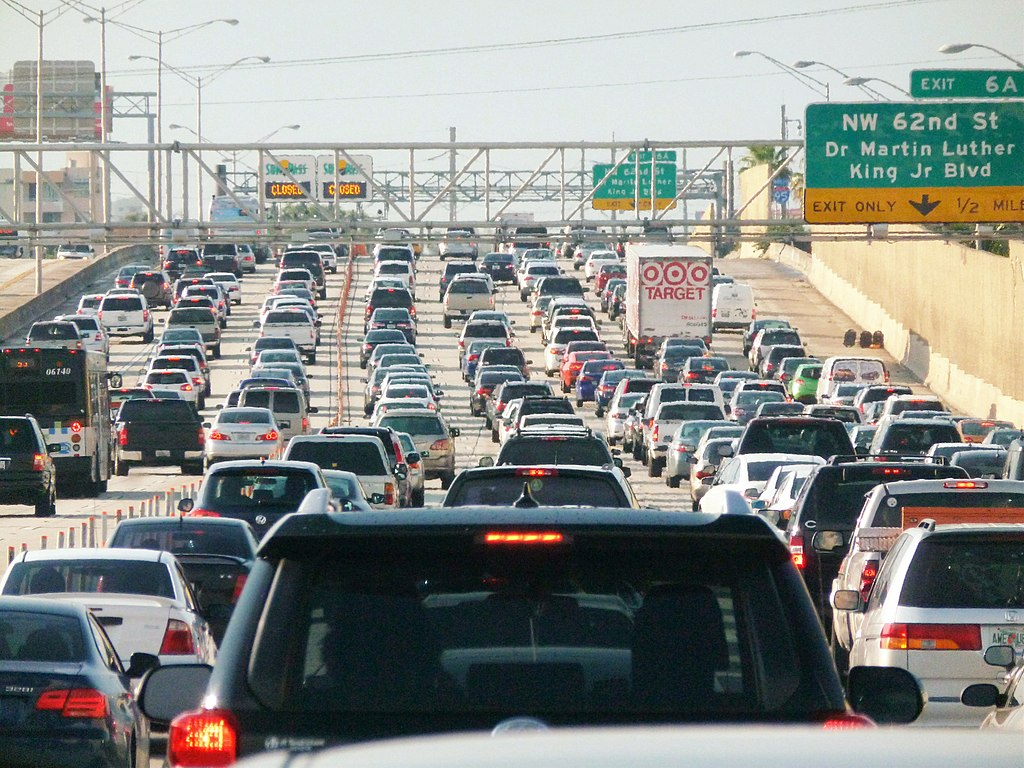
\includegraphics[width=0.5\textwidth]{figures/traffic.jpg}\\
		\hspace*{15pt}\hbox{\scriptsize Image By:\thinspace{\itshape B137}}
	\end{center}
	% https://commons.wikimedia.org/wiki/File:Miami_traffic_jam,_I-95_North_rush_hour.jpg
\end{frame}

\begin{frame}
	\frametitle{Me and my books}
	\framesubtitle{A life-long story cont'd}

	\begin{columns}
		\column{0.455\textwidth}
			\begin{center}
				\alt<4->{
					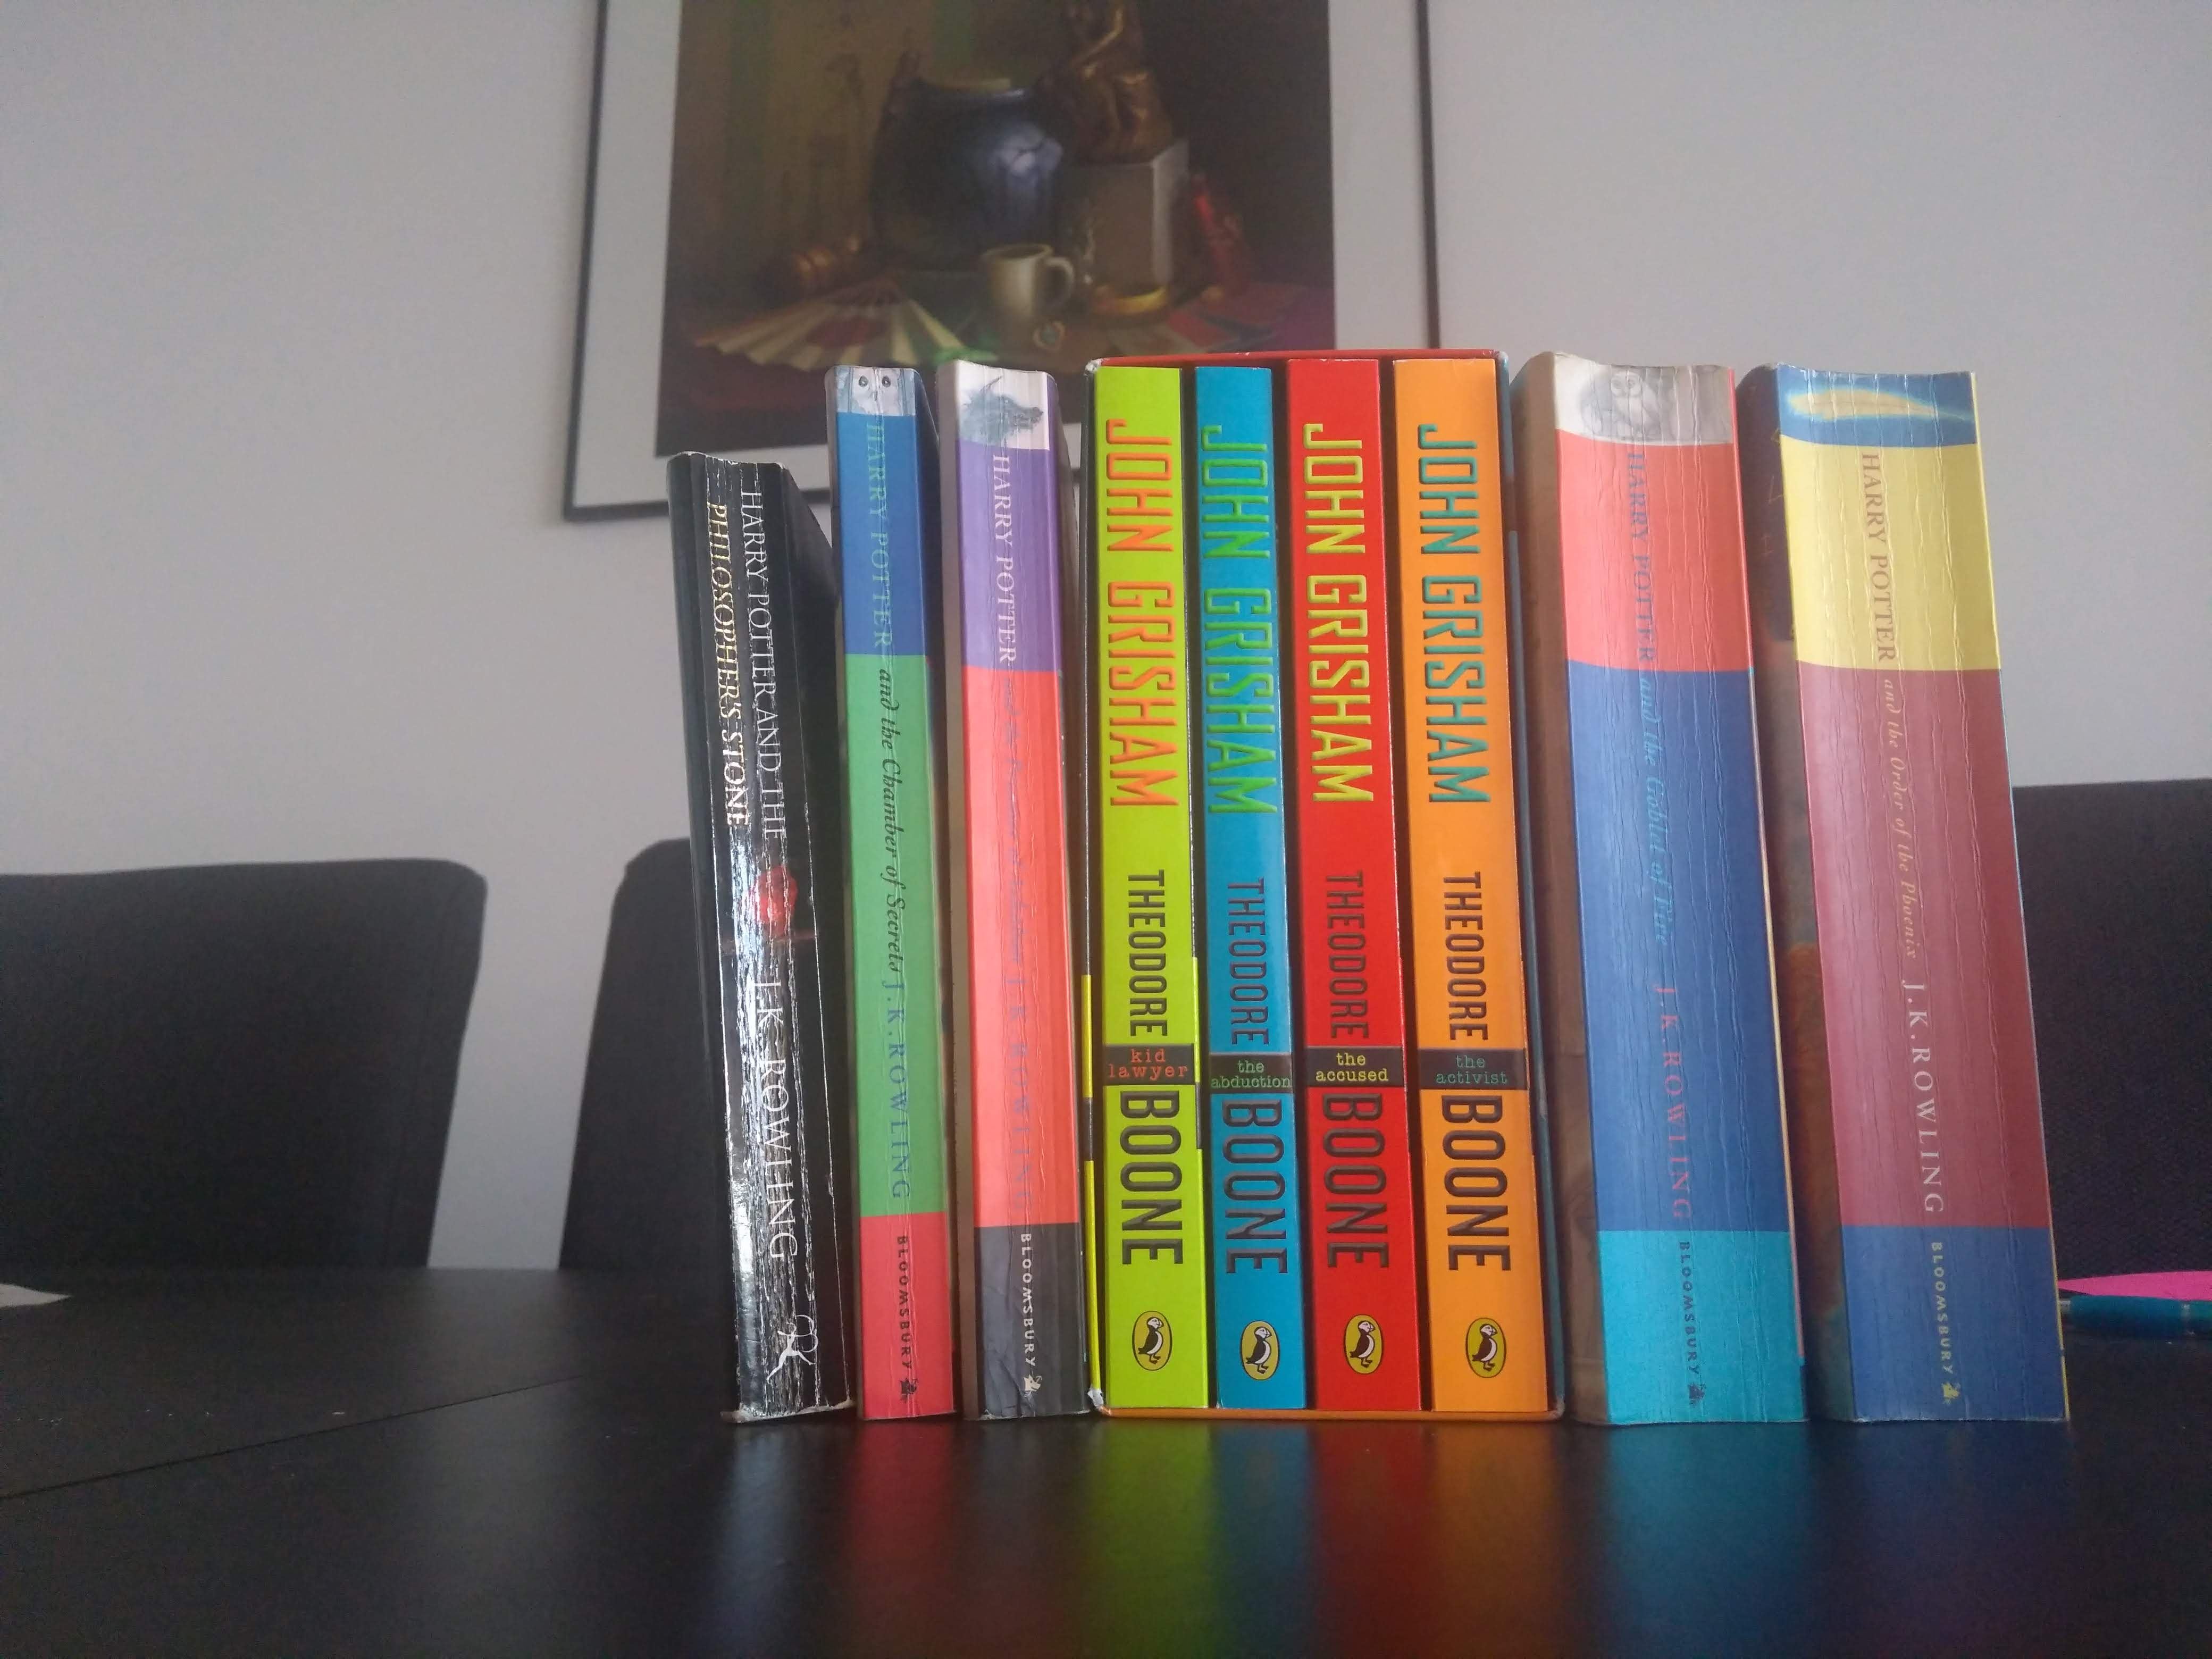
\includegraphics[width=\textwidth]{figures/queue_read.jpg}\\
					}{
					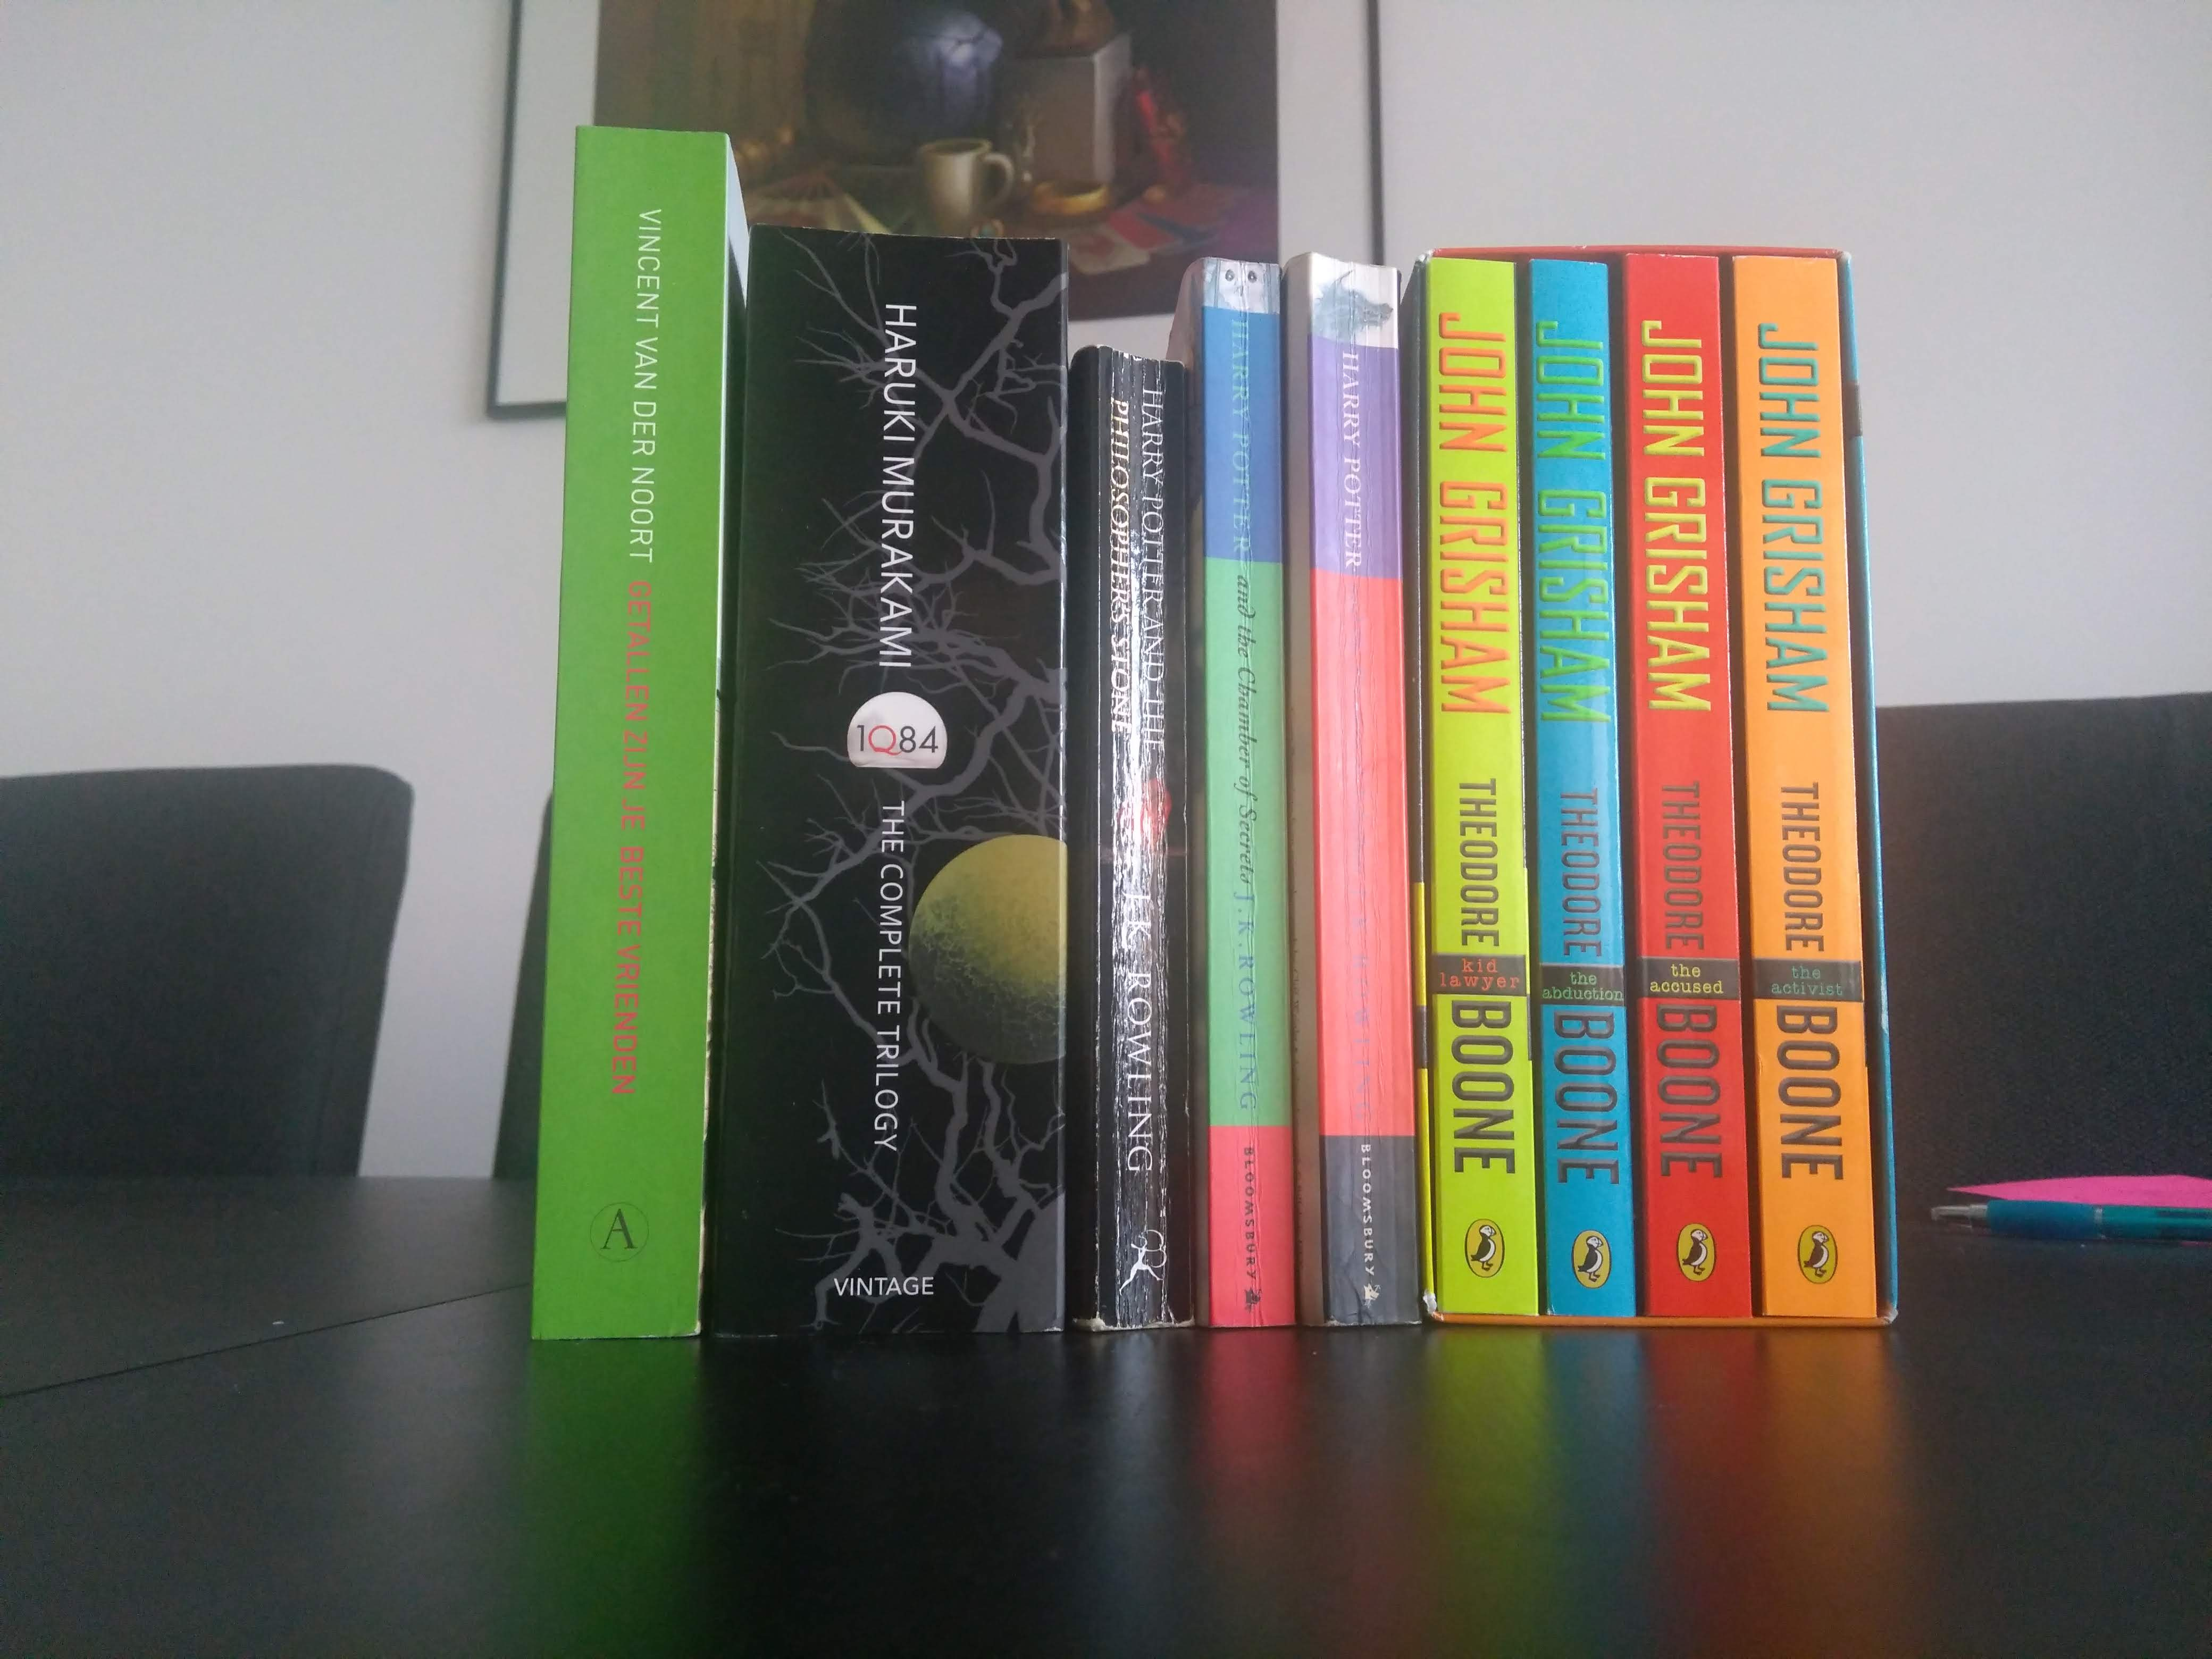
\includegraphics[width=\textwidth]{figures/queue_unread.jpg}\\
					}
				\hspace*{15pt}\hbox{\scriptsize Image By:\thinspace{\itshape Stefan Hugtenburg}}
				\hspace*{15pt}\hbox{\scriptsize Bookcovers and picture in the back by others}
			\end{center}
		\column{0.455\textwidth}
		\begin{itemize}
			\item This is how I now store books I still want to read.
				\pause
			\item A nice \alert{queue} of books, with new ones going on the right.
				\pause
			\item After finishing one, I take the next one from the left
				\pause
			\item So after a few weeks\dots
				\pause
			\item This uses the \alert{FIFO}-principle.
		\end{itemize}
	\end{columns}
\end{frame}

\begin{frame}
	\frametitle{The what!?}
	\framesubtitle{FIFO}
	
		\begin{block}{FIFO}
			The \textit{First-In-First-Out}, or FIFO, principle is the working of a queue.\\
			\pause
			The first thing we've added to the queue is the first thing we take out.\\
			\pause
			Similarly the last we have added to the queue, is the last to be taken out.
		\end{block}	
\end{frame}


\section{Intermezzo}
\label{sec:intermezzo}

\begin{frame}
	\frametitle{Intermezzo: Exams}
	\begin{center}
		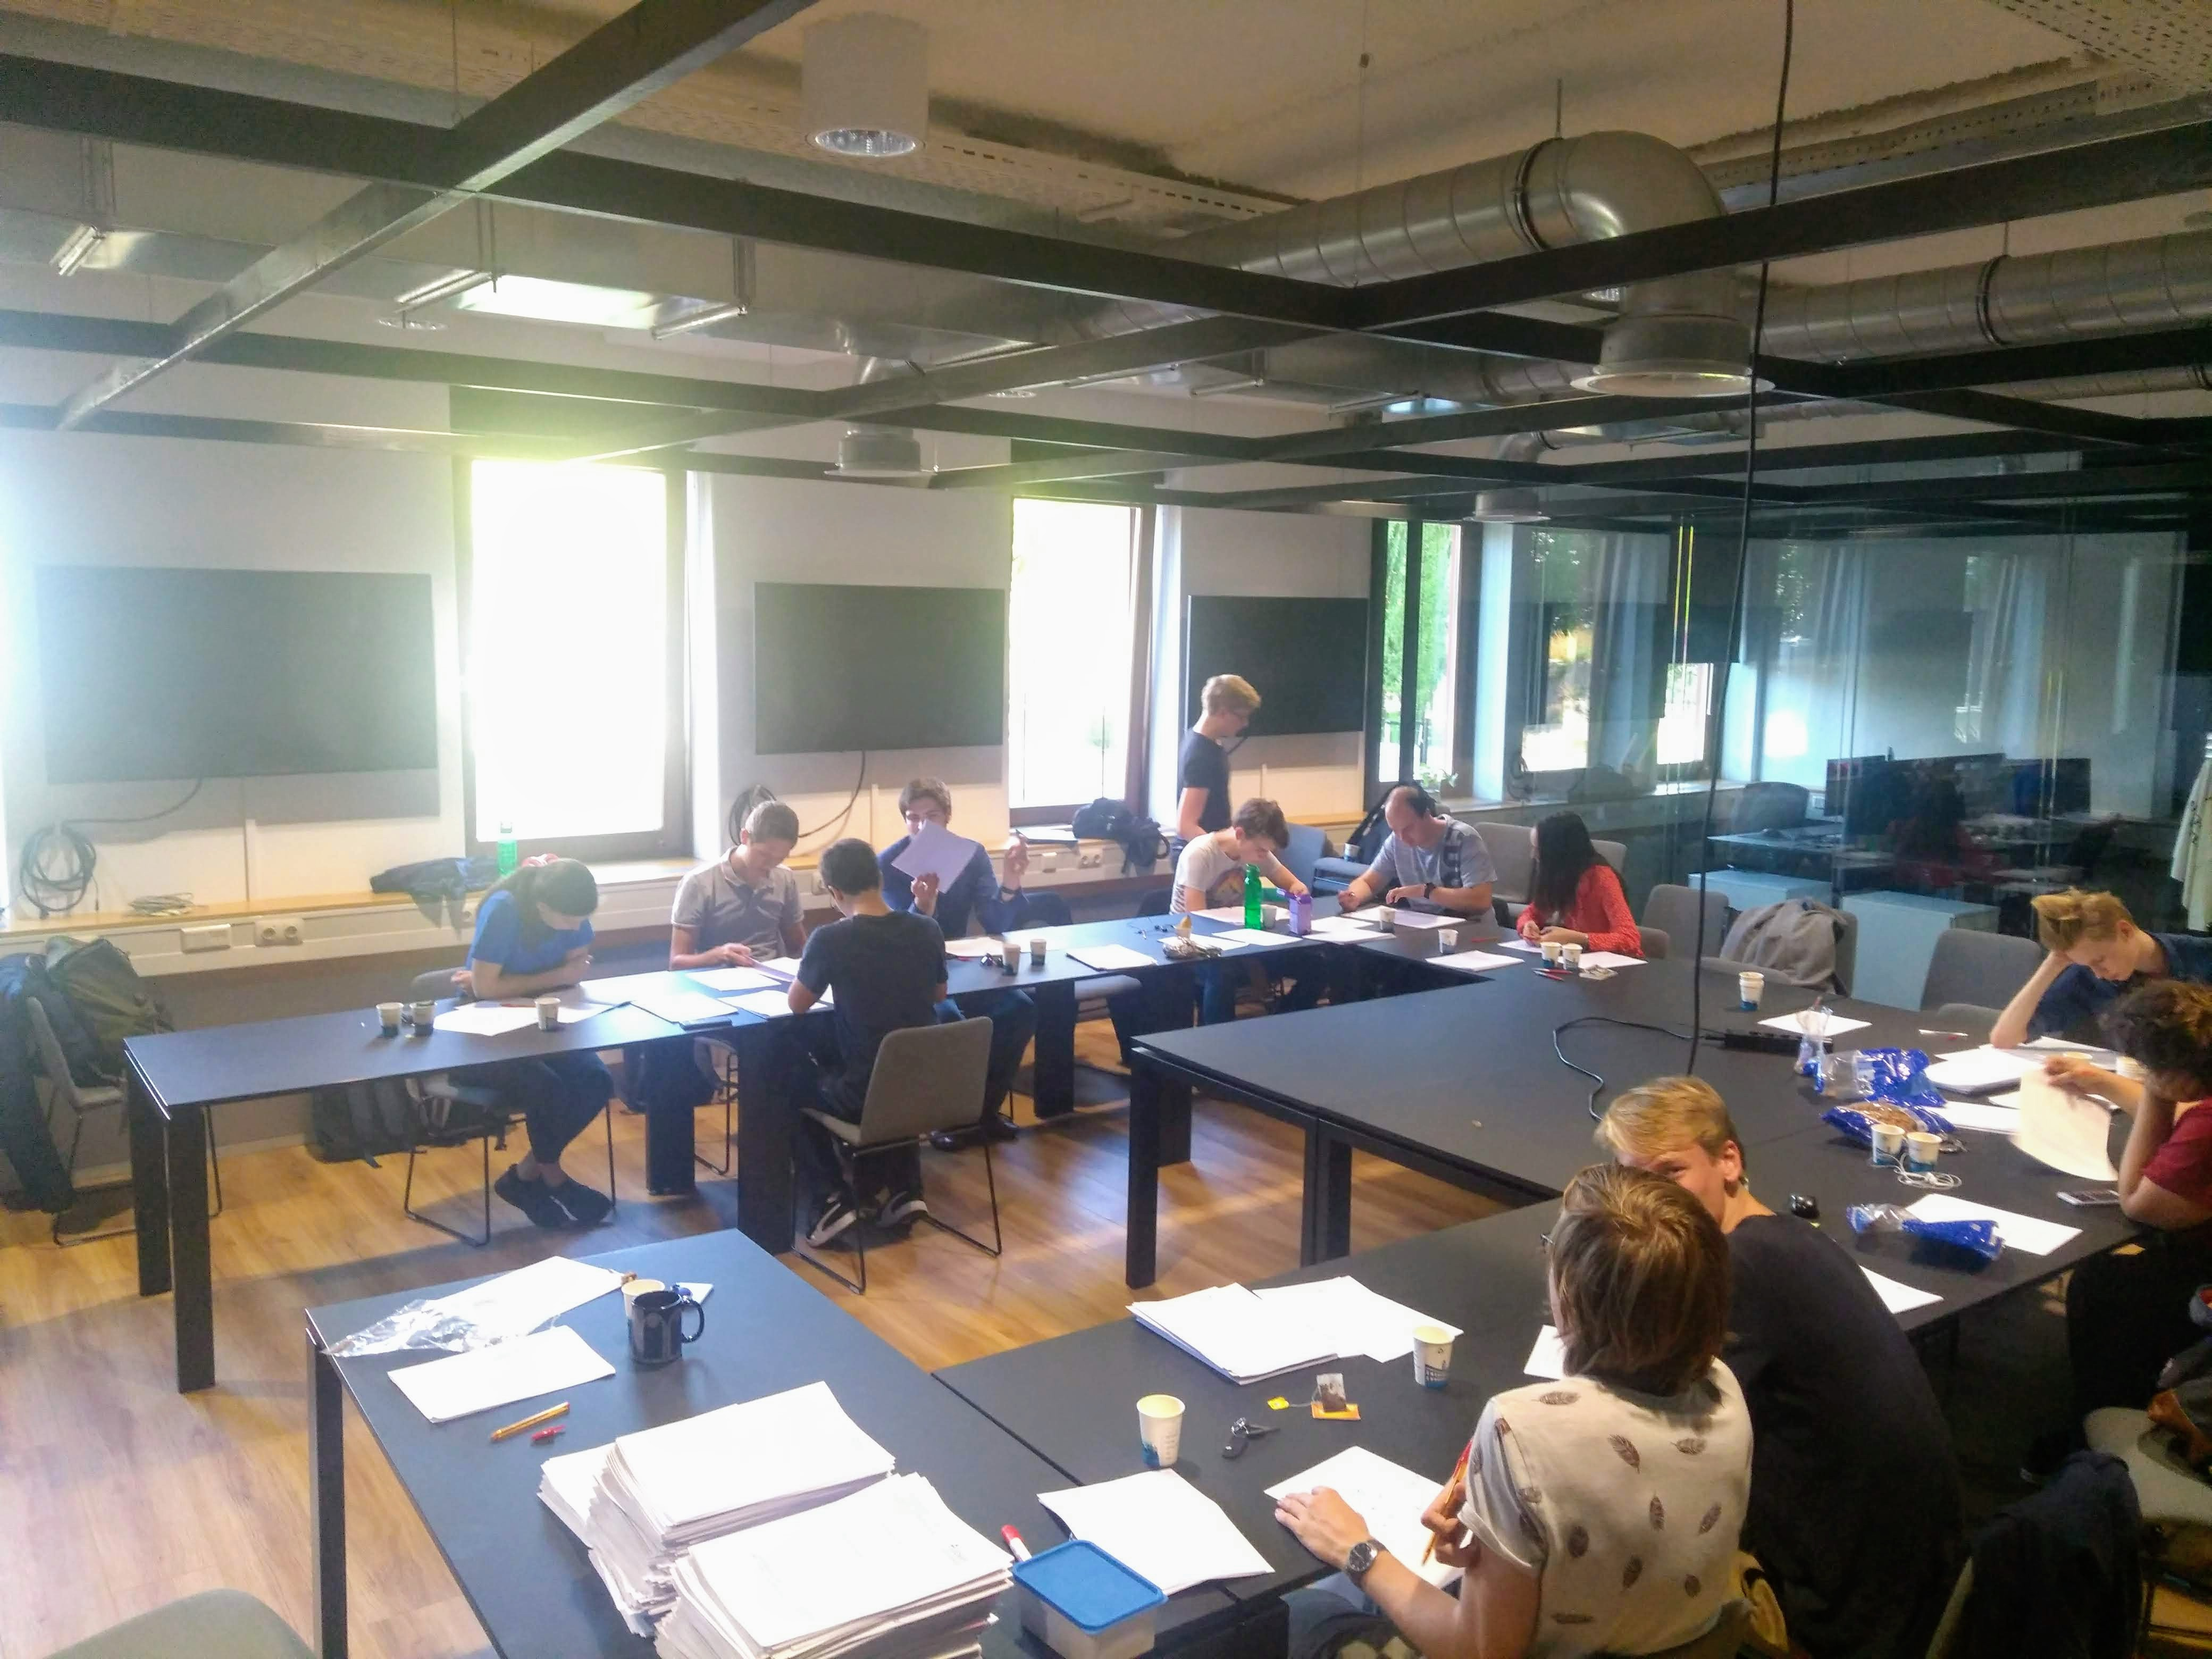
\includegraphics[width=0.6\textwidth]{figures/grading.jpg}\\
		\hspace*{15pt}\hbox{\scriptsize Image By:\thinspace{\itshape Stefan Hugtenburg}}
	\end{center}
\end{frame}

\begin{frame}
	\frametitle{The other type of tree}
	\framesubtitle{\url{https://science.howstuffworks.com/environmental/green-science/question16.htm}}
	\begin{itemize}
		\item We use a lot of paper, when it comes to exams\dots
			\pause
		\item Rough estimate of CSE first year, so far:
			\begin{itemize}
				\item 12 MC forms for 800 people
				\item 8 open question booklets for 800 people (2 sheets of paper each), assume everyone uses only one.
				\item 17 exams for 800 people, lets estimate that at 8 sheets each.
			\end{itemize}
			\pause
		\item	That's roughly 130-thousand sheets of paper.
			\pause
		\item Which is about 1.5 trees, according to howstuffworks.com
	\end{itemize}
\end{frame}

\begin{frame}
	\frametitle{Other interesting tree facts}
	\framesubtitle{\url{https://www.treesaregood.org/funfacts}}
	
	\begin{itemize}
		\item The oldest tree in the world is estimated at being 4765 years old.
			\pause
		\item The study of deteriming the age of a tree is called dendrochronology.
			\pause
		\item You are willing to pay more for goods and services if there are trees nearby! (slightly paraphrased)
			\pause
		\item Want to know more about where trees get their mass? Check this YouTube video:
			\url{https://www.youtu.be/2KZb2_vcNTg}
	\end{itemize}
\end{frame}


\begin{frame}
	\frametitle{The Queue ADT}
	\begin{overlayarea}{\textwidth}{\textheight}
		\begin{block}{The Queue}
			\begin{itemize}
				\item \texttt{size()} (or \texttt{len(s)}) to get the number of items in the queue.
				\item \texttt{enqueue(item)} to add something to the queue.
					\pause
				\item \texttt{dequeue()} to remove the first element from the queue.
				\item \texttt{peek()} to view the first element of the queue.
			\end{itemize}
		\end{block}	
		\pause
		\begin{questionblock}{Data structure?}
			What kind of data structure should we use to implement a Queue?
				\only<3>{
				\begin{enumerate}[A.]
					\item An array
					\item A python list
					\item A linked list
					\item A dict
				\end{enumerate}
			}
		\end{questionblock}
		\pause
		\begin{answerblock}{One end only}
			Only removing on one end and adding on the other? Seems like a DLL will do.
		\end{answerblock}
	\end{overlayarea}
\end{frame}

\begin{frame}
	\frametitle{Implementing a Linked-List based Queue}
	\begin{overlayarea}{\textwidth}{\textheight}
			\begin{tabular}{r | c c}
				Queue operation & DLL operation & Time Complexity \\
				\midrule
				\texttt{size} & \only<2->{\texttt{size} & $O(1)$} \\
				\texttt{enqueue} & \only<2->{\texttt{add\_last} & $O(1)$} \\
				\texttt{dequeue}  & \only<2->{\texttt{remove\_first} & $O(1)$} \\
				\texttt{peek}  & \only<2->{\texttt{head} & $O(1)$} \\
			\end{tabular}
		
			\begin{columns}[t]
				\column{0.455\textwidth}
			\only<3->{
			\begin{questionblock}{Arrays}
				Could we also do this using an array-based list?	
			\end{questionblock}
		}
			\only<5->{
			\begin{questionblock}{SLL}
				What about an SLL?
			\end{questionblock}
		}
				\column{0.455\textwidth}
				\only<4->{
				\begin{answerblock}{No more growing}
					Sure, but only for fixed capacity queues.
				\end{answerblock}
				}
				\only<6->{
				\begin{answerblock}{Eeyore}
					Only if we have the tail pointer.
				\end{answerblock}
				}
		
			\end{columns}
	\end{overlayarea}
\end{frame}

\begin{frame}
	\frametitle{Snake games}
	\framesubtitle{Nostalgia overload}
	\begin{center}
		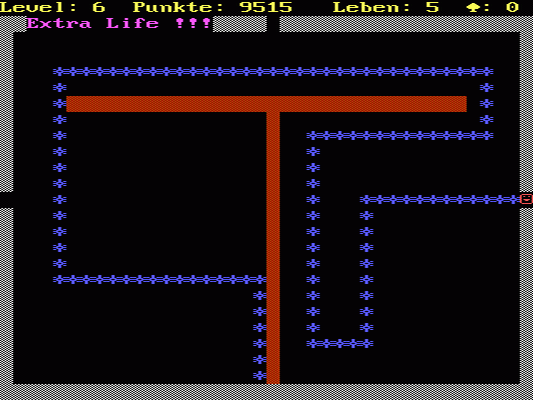
\includegraphics[width=0.6\textwidth]{figures/snake.png}\\
		\hspace*{15pt}\hbox{\scriptsize Image By:\thinspace{\itshape Thomas Jensen}}
	\end{center}
	% https://commons.wikimedia.org/wiki/File:Cgasnake.png 
\end{frame}

\begin{frame}
	\frametitle{Why a queue}
		\begin{block}{In snake...}
			\begin{itemize}
				\item In snake, the body of the snake follows the head.
					\pause
				\item If we first go left, then right, then every part of the body also needs to go first left then right.
					\pause
				\item This is like a queue!
			\end{itemize}
		\end{block}	
		\pause
			\begin{exampleblock}{Many others?}
				But of course there are many other real-world examples.
				\begin{itemize}
					\item Ticket counters,
					\item Traffic jams,
					\item Coffee machines and printers,
					\item Take-out restaurants,
					\item etc.
				\end{itemize}
			\end{exampleblock}	
\end{frame}


\begin{frame}
	\frametitle{Double-Ended Queues}

	\begin{center}
		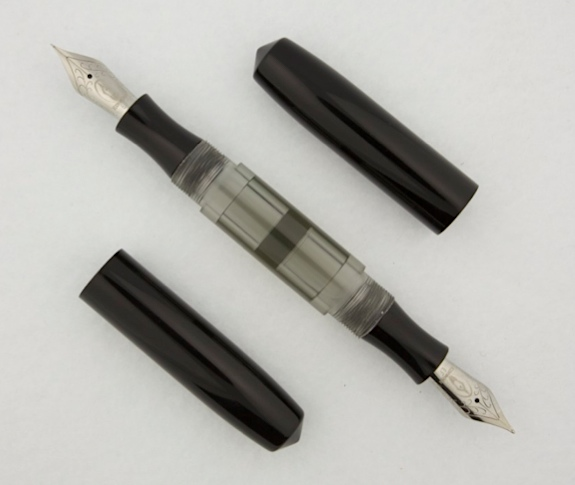
\includegraphics[width=0.5\textwidth]{figures/de.jpg}\\
		\hspace*{15pt}\hbox{\scriptsize Image By:\thinspace{\itshape Chris Lott}}
		% https://www.flickr.com/photos/fncll/9824392125
	\end{center}
\end{frame}

\begin{frame}
	\frametitle{Deques}
		\begin{block}{Deques}
			Deques, or Double-Ended Queues, allow both FIFO and LIFO operations in $O(1)$ time.
		\end{block}		
		\pause
		\begin{questionblock}{Hang on...}
			Doesn't that sound familiar?	
		\end{questionblock}
		\pause
		\begin{answerblock}{Back to DLL}
			This is exactly what a DLL offers!
		\end{answerblock}
\end{frame}

\begin{frame}
	\frametitle{\texttt{deque}}
	
	In python we can use a \texttt{deque} called \texttt{d} on which:
	\begin{itemize}
		\item We can \textit{push} with \texttt{d.append}.
		\item We can \textit{pop} with \texttt{d.pop}.
		\item We can \textit{top} with \texttt{d[-1]}
			\pause
		\item We can \textit{enqueue} with \texttt{d.append}.
		\item We can \textit{dequeue} with \texttt{d.popleft}.
		\item We can \textit{peek} with \texttt{d[0]}
			\pause
		\item Oh yeah and if you want, you can also add to the left with \texttt{appendleft}
	\end{itemize}
\end{frame}



\begin{frame}
\frametitle{A classic CS exercise}
\framesubtitle{Something hammer and nails?}	

\begin{problemblock}{Imagine...}
	Consider that we only have access to stacks, but I still want FIFO.\\
	What can I do?
\end{problemblock}
\pause
\begin{answerblock}{Create a stack-based queue}
	Create a queue out of two stacks!
\end{answerblock}
\end{frame}

\begin{frame}
	\frametitle{Let's get this started}
	
	\lstinputlisting{code/queuestack1.py}
	\begin{itemize}
		\item We will use two stacks to model the FIFO behaviour.
	\end{itemize}
\end{frame}

\begin{frame}
	\frametitle{Enqueueueueueing}
	\lstinputlisting{code/queuestack2.py}
	\begin{itemize}
		\item When adding, we just always add to \texttt{s1}.
			\pause
		\item The trick is in when we remove an item.
	\end{itemize}
\end{frame}

\begin{frame}
	\frametitle{Dequeueueueueing}
	\begin{questionblock}{How do we dequeue?}
		\begin{enumerate}[A.]
			\item We always \texttt{pop} from \texttt{s1}.
			\item We always \texttt{pop} from \texttt{s2}, when it is empty pop all of \texttt{s1} into \texttt{s2}.
			\item We always \texttt{pop} all of \texttt{s2} onto \texttt{s1}, then we pop from \texttt{s1}.
			\item I don't know.
		\end{enumerate}
	\end{questionblock}
\end{frame}

\begin{frame}
	\frametitle{Reverse when needed}
	\lstinputlisting{code/queuestack3.py}
\end{frame}

\begin{tikzpicture}[scale=0.85, transform shape]
	\only<3>{
		\foreach \x/\val in {0/1,1/20,2/42,3/22,4/17}{
			\node[draw,rectangle, fill=gray!10, minimum size =1cm] (c) at (\x,0) {\val};
		}
	}
	\only<4>{
		\foreach \x/\val/\col in {0/1/green,1/20/green,2/42/black,3/22/black,4/17/black}{
			\node[draw=\col,rectangle, fill=\col!10, minimum size =1cm] (c) at (\x,0) {\val};
		}
	}
	\only<5>{
		\foreach \x/\val/\col in {0/1/black,1/20/green,2/42/green,3/22/black,4/17/black}{
			\node[draw=\col,rectangle, fill=\col!10, minimum size =1cm] (c) at (\x,0) {\val};
		}
	}
	\only<6>{
		\foreach \x/\val/\col in {0/1/black,1/20/black,2/42/red,3/22/red,4/17/black}{
			\node[draw=\col,rectangle, fill=\col!10, minimum size =1cm] (c) at (\x,0) {\val};
		}
	}
	\only<7>{
		\foreach \x/\val/\col in {0/1/black,1/20/black,2/22/green,3/42/green,4/17/black}{
			\node[draw=\col,rectangle, fill=\col!10, minimum size =1cm] (c) at (\x,0) {\val};
		}
	}
	\only<8>{
		\foreach \x/\val/\col in {0/1/black,1/20/black,2/22/black,3/42/red,4/17/red}{
			\node[draw=\col,rectangle, fill=\col!10, minimum size =1cm] (c) at (\x,0) {\val};
		}
	}
	\only<9>{
		\foreach \x/\val/\col in {0/1/black,1/20/black,2/22/black,3/17/green,4/42/green}{
			\node[draw=\col,rectangle, fill=\col!10, minimum size =1cm] (c) at (\x,0) {\val};
		}
	}
	\only<10>{
		\foreach \x/\val/\col in {0/1/green,1/20/green,2/22/black,3/17/black,4/42/black}{
			\node[draw=\col,rectangle, fill=\col!10, minimum size =1cm] (c) at (\x,0) {\val};
		}
	}
	\only<11>{
		\foreach \x/\val/\col in {0/1/black,1/20/green,2/22/green,3/17/black,4/42/black}{
			\node[draw=\col,rectangle, fill=\col!10, minimum size =1cm] (c) at (\x,0) {\val};
		}
	}
	\only<12>{
		\foreach \x/\val/\col in {0/1/black,1/20/black,2/22/red,3/17/red,4/42/black}{
			\node[draw=\col,rectangle, fill=\col!10, minimum size =1cm] (c) at (\x,0) {\val};
		}
	}
	\only<13>{
		\foreach \x/\val/\col in {0/1/black,1/20/black,2/17/green,3/22/green,4/42/black}{
			\node[draw=\col,rectangle, fill=\col!10, minimum size =1cm] (c) at (\x,0) {\val};
		}
	}
	\only<14>{
		\foreach \x/\val/\col in {0/1/black,1/20/black,2/17/black,3/22/green,4/42/green}{
			\node[draw=\col,rectangle, fill=\col!10, minimum size =1cm] (c) at (\x,0) {\val};
		}
	}
	\only<15>{
		\foreach \x/\val/\col in {0/1/green,1/20/green,2/17/black,3/22/black,4/42/black}{
			\node[draw=\col,rectangle, fill=\col!10, minimum size =1cm] (c) at (\x,0) {\val};
		}
	}
	\only<16>{
		\foreach \x/\val/\col in {0/1/black,1/20/red,2/17/red,3/22/black,4/42/black}{
			\node[draw=\col,rectangle, fill=\col!10, minimum size =1cm] (c) at (\x,0) {\val};
		}
	}
	\only<17>{
		\foreach \x/\val/\col in {0/1/black,1/17/green,2/20/green,3/22/black,4/42/black}{
			\node[draw=\col,rectangle, fill=\col!10, minimum size =1cm] (c) at (\x,0) {\val};
		}
	}
	\only<18>{
		\foreach \x/\val/\col in {0/1/black,1/17/black,2/20/green,3/22/green,4/42/black}{
			\node[draw=\col,rectangle, fill=\col!10, minimum size =1cm] (c) at (\x,0) {\val};
		}
	}
	\only<19>{
		\foreach \x/\val/\col in {0/1/black,1/17/black,2/20/black,3/22/green,4/42/green}{
			\node[draw=\col,rectangle, fill=\col!10, minimum size =1cm] (c) at (\x,0) {\val};
		}
	}
	\only<20>{
		\foreach \x/\val/\col in {0/1/green,1/17/green,2/20/black,3/22/black,4/42/black}{
			\node[draw=\col,rectangle, fill=\col!10, minimum size =1cm] (c) at (\x,0) {\val};
		}
	}
	\only<21>{
		\foreach \x/\val/\col in {0/1/black,1/17/green,2/20/green,3/22/black,4/42/black}{
			\node[draw=\col,rectangle, fill=\col!10, minimum size =1cm] (c) at (\x,0) {\val};
		}
	}
	\only<22>{
		\foreach \x/\val/\col in {0/1/black,1/17/black,2/20/green,3/22/green,4/42/black}{
			\node[draw=\col,rectangle, fill=\col!10, minimum size =1cm] (c) at (\x,0) {\val};
		}
	}
	\only<23->{
		\foreach \x/\val/\col in {0/1/black,1/17/black,2/20/black,3/22/green,4/42/green}{
			\node[draw=\col,rectangle, fill=\col!10, minimum size =1cm] (c) at (\x,0) {\val};
		}
	}
\end{tikzpicture}

\begin{frame}
	\frametitle{You are here.}
	\begin{block}{The course so far}
		\begin{itemize}
			\item Time and Space complexity
			\item Lists, Stacks, and Queues
			\item Sorting
		\end{itemize}
	\end{block}
	\pause
	\begin{exampleblock}{Today's content}
		\begin{itemize}
			\item Trees!
			\item Properties and traversals
		\end{itemize}
	\end{exampleblock}
	\pause
	\begin{block}{The future}
		\begin{itemize}
			\item Heaps and Search Trees
			\item Maps, Sets, and Graphs
			\item P vs NP\dots
		\end{itemize}
	\end{block}
\end{frame}

\begin{frame}
	\frametitle{Homework for this week}
	\begin{itemize}[<+->]
		\item \alert{After} today's lecture: read the Chapter 8.
		\item \alert{Before} Friday, check out the example exam (so that you can ask questions).
		\item \alert{Before} Sunday, do the homework :)
	\end{itemize}
\end{frame}

\begin{frame}
	\frametitle{Mudcards}
	\framesubtitle{\url{https://www.delta.tudelft.nl/article/column-van-koelkasten-kranen-en-college}}

	\begin{block}{Based on a column by Bob van Vliet}
		\begin{itemize}
			\item At the end of every lecture, a short (2-question) survey.
			\item Tell me one thing you liked.
			\item And one thing you didn't like.
			\item Be concrete, be specific!
		\end{itemize}
	\end{block}
\end{frame}



\frame{\titlepage}

\end{document}
